
\documentclass[12pt]{article}
\usepackage{rotating}
\usepackage{amsmath}
\usepackage{graphicx}
\usepackage{verbatim}
\usepackage{caption}
\usepackage{subcaption}
\usepackage{setspace}
\usepackage{color}
\usepackage{amsfonts}
\usepackage{amssymb}
\usepackage{float}
\usepackage{lscape}
\usepackage{ulem}
\usepackage{soul}
%\usepackage{bbm}
\usepackage[authoryear,round]{natbib} 
\usepackage[colorlinks=true,
linkcolor=blue,
anchorcolor=blue,
citecolor=blue,
urlcolor =blue]{hyperref}
\usepackage{makecell}
\usepackage{appendix}
\usepackage{minitoc}
\hypersetup{
colorlinks=true,
linkcolor=blue,
anchorcolor=blue,
citecolor=blue}
%\hypersetup{hidelinks} % hide the ugly red box in footnote links
\setcounter{MaxMatrixCols}{30}
\providecommand{\U}[1]{\protect\rule{.1in}{.1in}}
\pagestyle{plain}
%\setcitestyle{authoryear,round}
\usepackage[margin=1truein]{geometry}
\newtheorem{theorem}{Theorem}
\newtheorem{acknowledgement}[theorem]{Acknowledgment}
\newtheorem{algorithm}{Algorithm}               
\newtheorem{axiom}{Axiom}
\newtheorem{case}{Case}
\newtheorem{claim}{Claim}
\newtheorem{conclusion}{Conclusion}
\newtheorem{condition}{Condition}
\newtheorem{conjecture}{Conjecture}
\newtheorem{corollary}{Corollary}
\newtheorem{criterion}{Criterion}
\newtheorem{definition}{Definition}
\newtheorem{example}{Example}
\newtheorem{exercise}{Exercise}
\newtheorem{lemma}{Lemma}
\newtheorem{notation}{Notation}
\newtheorem{problem}{Problem}
\newtheorem{proposition}{Proposition}
\newtheorem{remark}{Remark}
\newtheorem{solution}{Solution}
\newtheorem{summary}{Summary}
%\doublespacing
\onehalfspacing
\graphicspath{{figure/}}
\newenvironment{proof}[1][Proof]{\textbf{#1.} }{\ \rule{0.5em}{0.5em}}
\RequirePackage{threeparttable}
\RequirePackage{booktabs}
\RequirePackage{tabularx}
%\graphicspath{{figure/}}
\makeatletter\let\ExpandableInput\@@input\makeatother
% defines ExpandableInput command which solves the
% problem of having noalign problem in the first line
% of input tables
\def\sym#1{\ifmmode^{#1}\else\(^{#1}\)\fi}  % defines
% the superscripts in tables (significance stars)
\begin{document}

\title{Does Pollution Affect Exports? Evidence from China\thanks{%
We benefit from presentations at Asia-Pacific Trade Seminars (2022) and International Symposium on
Trade and Green Environment (2023).}}
\author{Jie Bai\thanks{%
Department of Economics, Lingnan University, Hong Kong, E-mail: jiebai@ln.hk}
\quad Larry D. Qiu\thanks{%
Department of Economics, Lingnan University, Hong Kong, E-mail:
larryqiu@ln.edu.hk} \quad Junji Xiao\thanks{%
Department of Economics, Lingnan University, Hong Kong, E-mail:
junjixiao@ln.edu.hk.}}
\date{March 1, 2023}

\maketitle

\begin{abstract}
The literature on the correlation between trade and environment is vast, but
studies almost exclusively focus on the causal effects of trade on
environment. This study examines the reverse effects. We use Chinese export
and pollution data, at firm and county levels, over the period of 2000 $-$ 2007
to investigate whether and how air pollution affects firms' exports. Using $%
\mathrm{PM_{2.5}}$ concentrations as a proxy for air pollution and employing
thermal inversion as an instrumental variable, we find that a 1\% increase
in $\mathrm{PM_{2.5}}$ leads to a 0.79\% reduction in firms' exports. This
adverse effects of air pollution on exports are mainly attributed to the
intensive margins as opposed to the extensive margins. Our mechanism
analysis identifies two channels: (1) air pollution decreases exports by
reducing firm productivity, and (2) air pollution invites stringent
environmental regulations, which reduces exports as firms need to increase
abatement costs or reduce production to meet the environment standards.
\end{abstract}

\begin{quote}
\emph{Keywords:} Export; Air Pollution; Productivity; Environmental 
Regulation 

\emph{JEL Classification:} F14, F18, Q51 
\end{quote}

\newpage  \setcounter{page}{1} 

\section{Introduction}

\label{sec:1} Rapid trade and economic growth are usually accompanied by
environmental deterioration especially in developing countries such as
China. For example, during the rapid growth period from 2000 to 2007, air quality in China deteriorated substantially:
 the annual average $\mathrm{PM_{2.5}}$
concentration increased from 44 $\mu g/m^{3}$ to 56.71 $\mu g/m^{3}$, far exceeding the World Health Organization
(WHO) air quality
guideline (10 $\mu g/m^{3}$).\footnote{%
For fine particulate matter ($\mathrm{PM_{2.5}}$), WHO published Global Air Quality Guidelines (AQG) in 2005 and recommend not exceeding 10 $\mu g/m^{3}$ for annual mean and 25 $\mu g/m^{3}$ for 24-hour mean.
See %
\url{https://www.who.int/news-room/feature-stories/detail/what-are-the-who-air-quality-guidelines}
for more information.} This causes serious
concerns about the balance between environment and economic development. There exists
a large body of research and evidence showing that trade and economic growth cause
pollution.\footnote{%
See \cite{cherniwchan2017trade} for the most recent survey of the literature.%
} An equally interesting question is whether pollution reduces economic and
trade growth. Recent empirical evidence has shown that severe pollution
reduces labor productivity through harming people's health while health is a crucial part of human capital %
\citep{graff2012impact,chang2016particulate,zhang2018impact,fu2021air,somanathan2021impact,adhvaryu2022management}%
. In this paper, we ask a different but related question: does pollution
influence international trade and how? We explore this question based on the
evidence of China, which has experienced rapid increases in both trade and
pollution.

A big challenge in the empirical studies of the causal effects between trade
and environment is the endogeneity problem. This problem is more serious in
the identification of pollution effects on trade than that of trade effects on
pollution, because in the latter case, researchers often find good
instrumental variables (IVs) for trade, such as trade agreements and trade shocks.
In this study, we overcome the endogeneity problem using the IV method to examine the causal impact of air pollution on firms'
exports. In particular, following the environmental economics literature 
\citep[e.g.,][]{fu2021air,
fu2021trans,NBERw28401,chen2022effect}, we use thermal inversions (in
the main analysis) or wind directions (in robustness check) respectively,
as IVs for $\mathrm{PM_{2.5}}$ concentration, which is one of the important measures
for air pollution, at the county level, to study the effects of
pollution on individual firms' exports in China from 2000 to 2007. Thermal
inversion is a reversal of the normal behavior of temperature in the
atmosphere nearest the earth's surface. It is a phenomenon caused by
meteorological factors rather than economic activities. When it occurs, air
pollution is trapped close to the ground and thus increases.

Applying the two-stage least squares (2SLS) estimation method to our empirical analysis,
% We use 2SLS estimation method with thermal inversion as the instrumental
% variable for air pollution in our empirical analysis. We 
we find that air
pollution reduces exports at both intensive and extensive margins.
Specifically, following an 1\% increase in $\mathrm{PM_{2.5}}$ concentration,
the firms' export values decrease by 0.79\% on average, their
probabilities of entering foreign markets decrease by 0.06\%,
while their probabilities of exiting the foreign markets increase by
0.15\%. 
% In searching for the channel through which air
% pollution reduces exports, we first find 
The mechanism analysis suggests that the adverse effects of air pollution on exports are mediated by firm productivity and moderated by environmental regulations. Our empirical results show
that air pollution has detrimental
effects on labor productivity and total factor productivity (TFP), echoing
the recent findings in the environmental economics literature %
\citep{NBERw18392,fu2021air,NBERw28401}. Together with the well-documented findings in the
trade literature  that productivity is an important determinant of exports,
this suggests that productivity is a possible mediator of air
pollution impact on exports. We confirm this channel in our study. In
addition, we also find that the negative effects of air pollution on exports
are more significant in the regions with tighter pollution regulations. This finding is consistent with the recent evidence from the
studies on how environmental regulations affect exports \citep[e.g.,][]{
cherniwchan2022environmental} and suggests another channel through which air
pollution reduces exports: Stringent environmental policies raise the costs
of production, by increasing costs on abatement technology or forcing
reduction of production, which in turn reduces exports. We conduct further
empirical analyses on the heterogeneous effects which provide indirect
evidence to support the above two channels.

This paper makes significant contributions to the literature of the interplay between
international trade and environment. There exist several review articles of
this literature including \cite{cherniwchan2017trade} and \cite{NBERw30020}
as the most recent ones. Almost all existing studies focus on how
international trade affects pollution. A general conclusion from these
studies is that trade liberalization impacts pollution via the scale,
composition, and technique effects \citep{NBERw3914,copeland1994north}. Our
paper clearly differs from this strand of literature as we examine the
opposite direction of the effects: how pollution affects trade.

Although they are scant, there exist a few studies that examine the effects
of environmental factors on trade. \cite{jones2010climate} find that higher
temperatures in poor countries have large and negative impacts on the growth
of their agricultural and light manufacturing exports. \cite%
{dellink2017international} describe the potential channels through which
climate change damages trade. The channels include the direct impact on
transport and distribution chains and the indirect influences on factors of
production. Our paper adds to these studies by documenting rare empirical evidence
%is closely related to this line of studies to study
% the effects of environment on trade, 
% but unlike these papers, we conduct a
% rigorous empirical analysis of the effects 
of air pollution on exports,
based on the Chinese firm-level data.

Our mechanism analysis of the pollution effects on exports contributes to 
% As mentioned earlier, the two mechanisms that we identify in the air
% pollution's effects on exports are productivity and environmental
% regulations. This part of analysis is related to 
two strands of literature.
The first strand of literature studies the effects of pollution on productivity.
Existing research has shown that various types of air pollution (e.g.,
ozone, $\mathrm{PM_{2.5}}$) have negative impacts on productivity %
\citep{graff2012impact,chang2016particulate,fu2021air,adhvaryu2022management}
% For example, based on the Chinese data from 1998 to 2007, \cite{fu2021air} use
% thermal inversions as an instrument to find that a decrease in $\mathrm{%
% PM_{2.5}}$ increases productivity in China's manufacturing sector.\ 
Our study goes one step further to show that the undermined productivities caused by air pollution finally 
% air pollution reduces productivity,
% which in turn 
reduce firms' exports.

The second strand of literature studies the effects of environmental regulations on
exports.\footnote{%
Several papers investigate the effects of environmental regulations on
foreign direct investment \citep{dean2009foreign,cai2016does}.} \cite%
{hering2014environmental} study the Two-Control-Zones policy in China and
find that exports significantly decrease in targeted cities and fall more
sharply in pollution-intensity industries. \cite{shi2018environmental} show
that the policy that sets pollution reduction targets in China's Eleventh
Five-Year Plan results in exports fall in targeted cities. Different from
these studies, our paper focuses on the effects of pollution \textit{per se}
on exports. However, these studies inspire us to find the second channel of
the pollution's impact on exports, namely, the environmental regulations' mediation effects.%
\footnote{%
There exists another, but less relevant, literature of the effects of
environmental regulations on productivity. \cite{berman2001environmental}
find that TFP rises in air quality regulation regions as abatement
investment appear to be productivity enhancing in the US. \cite{NBERw18392}
find that stricter air quality regulations are associated with a roughly
2.6\% decline in TFP in the US. \cite{he2020watering} find that a water
quality regulation campaign in China significantly reduces upstream
polluting firms' TFP by more than 24\% compared to downstream.}

The rest of the paper is organized as follows. We specify our empirical
strategy in Section \ref{sec:empirical_strategy}. We describe our data and measurements in Section \ref{sec:3}.
We present the main empirical findings in Section \ref{sec:4} and explore the
mechanisms in Section 5. We provide concluding remarks in Section 6.

\section{Empirical Model and Identification}

\label{sec:empirical_strategy} This section presents our empirical
methodology of estimating the impact of air pollution on individual firms'
exports. Two-stage
least squares (2SLS)
estimation is applied to solve the potential endogeneity problem with
air pollution.

\subsection{Empirical Model}

To investigate the impact of air pollution on firms' exports, we assume
exports to be a function of pollution; moreover, we control for the major
determinants of exports. Specifically, letting $Export_{ict}$
denote the value of exports by firm $i$ from county $c$ in year $t$, we
assume 
\begin{equation}
ln(Export_{ict})=\beta _{0}+\beta _{1}ln(P_{ct})+\mathbf{X}%
_{ict}^{^{\prime }}\Gamma +\mathbf{W}_{ct}^{^{\prime }}\beta _{w}+\delta
_{i}+\lambda _{t}+\epsilon _{ict}.  \label{equ1}
\end{equation}%
In the above equation, $ln(Export_{ict})$ is the natural
logarithmic value of exports. $ln(P_{ict})$ is the logarithmic air
pollution density. The vector $\mathbf{X}_{ict}^{^{\prime }}$ consists of
variables measuring firm characteristics, including age, size,
capital stock, and productivity. 

Productivity is measured by either labor
productivity or revenue-based TFP. Labor productivity is defined as the
ratio of the firm's value added to the number of employees. We estimate TFP
using both Levinsohn-Petrin method \citep{levinsohn2003estimating} and
Olley-Pakes method \citep{olley1996dynamics}, denoted as $TFP_{LP}$ and $%
TFP_{OP}$, respectively. TFP is estimated using the output data at four-digit
Chinese standard industrial classification (CSIC), considering heterogeneous
productivity across industries. All measures of productivity are in
logarithmic form and are deflated by respective price index developed by %
\citep{brandt2017wto}. 

As the previous literature %
\citep[e.g.,][]{jones2010climate} suggests that weather may affect exports,
we also control for weather, represented by vector $\mathbf{W}%
_{ct}^{^{\prime}}$, which includes temperature, precipitation, humidity,
wind speed, and sunshine duration. 

Various fixed effects are also controlled in our regression. $\lambda _{t}$ is the time fixed effects,
capturing the time trends and all other possible time-specific shocks such
as annual socioeconomic cycles that may affect exports. $\delta _{i}$ is the
firm fixed effects. Since few
firms switch industries, so all time-invariant, industry-specific
unobservable affecting exports are absorbed by the firm fixed effects.\footnote{Only 4\% of firms relocate counties during the sample period, so that controlling for firm fixed effects is sufficient. We provide robustness check in the Appendix.}

The error term, $\epsilon _{ict}$, is assumed to be mean zero and independent across
firms, clustering at firm-level, permitting correlation in outcomes across pollution density
within the same firm. We list the definitions of the key variables in Table~\ref%
{tab:var_definition} for easy reference.

\begin{center}
$<$Table~\ref{tab:var_definition} Here$>$
\end{center}

\subsection{Identification Strategy: Instrument Variables}
Applying the ordinary least square (OLS) estimation method to Eq.(\ref{equ1}%
) will provide the correlation between pollution and exports. However, the
OLS estimators are biased due to endogeneity problems with pollution caused by reverse
causality and omitted variables. For instance, the increased exports may come from the changes in production technology, which increases productivity at the cost of more air pollution. 
% more production which generates more pollution.
% Introduction of new production technologies can affect both export and air quality. 
We adopt an IV strategy to address these empirical challenges. Following the literature on environmental economics %
\citep{arceo2016does,jans2018economic,sager2019estimating,fu2021air}%
, we use county-level days of thermal inversions per annum as the
IV. In the first stage of the 2SLS, we regress air
pollution density $ln(P_{ct})$
on thermal inversion, denoted as $TI_{ct}$, controlling for the same variables as in Eq.(\ref{equ1}):


  \begin{equation}  \label{equ2}
    ln(P_{ct}) = \alpha_{0} + \alpha_{1}TI_{ct} + \alpha_{2}\mathbf{W}%
    _{ct} + \mathbf{X}^{^{\prime }}_{ict}\Phi + \delta_{i} + \lambda_{t} + \mu_{
    ict}
    \end{equation}

Then, in the second stage of the 2SLS, we run regression based on Eq.(\ref%
{equ1}) but with the key explanatory variable $ln(P_{ct})$ replaced by the
estimated one obtained from Eq.(\ref{equ2}).

As described by \cite{jacobson2002atmospheric} and \cite{arceo2016does},
thermal inversion is a reversal of the normal behavior of temperature in
the troposphere, which is the region of the atmosphere nearest Earth's
surface. Under normal conditions, air temperature usually decreases with
height. When a layer of cool air at the surface of the troposphere is
overlain by a layer of warmer air, which acts as a cap on the upward
movement of the air from the layers below, a thermal inversion occurs (see
Fig.~\ref{fig:1}). Consequently, convection caused by the heating of the air
from below is limited to levels below the inversion and so air pollution is
trapped close to the ground due to thermal inversion. This positive
correlation between air pollution and thermal inversion is owing to
meteorological factors.

\begin{center}
$<$Figure~\ref{fig:1} Here$>$ 
\end{center}

Thermal inversion typically occurs for three reasons. First, thermal inversion
occurs when there is a high pressure system and air from high pressure
center in the atmosphere sinks down to fill the space left as air blows
outward, resulting in a layer of hot air on a layer of cold. Second, thermal
inversion can happen when air moves horizontally and a warm air layer is
squeezed upwards onto the cold denser air. Third, thermal inversion
happens when air temperature near the ground cools down faster than that in
the air above, resulting in the temperature near the ground lower than that
in the upper layers. 

Because thermal inversion is a pure meteorological phenomenon that affects
pollution but is unlikely to directly affect other economic and social
activities, it has become a popular IV for pollution in
empirical studies %
\citep{arceo2016does,jans2018economic,sager2019estimating,chen2022effect,NBERw28401}%
. It is also a valid IV in our study because it satisfies
the following two conditions: Relevance (correlation) and exogeneity (exclusion). First,
as we describe above, when a thermal inversion occurs, pollutants are
trapped in the air close to the ground, and thus, pollution level increases.
Hence, the number of thermal-inversion days observed in a year must be positively
correlated with the average pollution level of the year. We confirm this positive correlation later based on our data of thermal inversions and $\mathrm{PM_{2.5}}$ at the county-year level in China. Thus, the relevance condition is satisfied.

  Second, no evidence suggests that thermal inversions are correlated with
  exports. Thermal inversions are driven by meteorological factors but not by
  socioeconomic factors, and so they are not correlated with economic activities
  such as exports. Hence, our IV satisfies the exclusion restriction. We confirm this later with the evidence based on our data of
  thermal inversions at the county-year level in China. 
  
  \section{Data and Measurement}

  \label{sec:3}
  
  \subsection{Air Pollution}
  \label{sec:3.1} 
  Various measures of air pollution are available. The US Environmental Protection Agency has
  identified six pollutants as \textquotedblleft criteria\textquotedblright\
  air pollutants, including carbon monoxide, lead, nitrogen oxides,
  ground-level ozone, particle pollution (often referred to as particulate
  matter), and sulfur oxides. These pollutants are found to harm human health
  and the environment. Among these pollutants, the particulate pollutant that
  is 2.5 microns or smaller in size, called $\mathrm{PM_{2.5}}$, is widely used in
  the literature as an index for air pollution %
  \citep[e.g.,][]{chang2016particulate,fu2021air}. Following this literature, we also
  use $\mathrm{PM_{2.5}}$ concentration to measure air pollution.
  
  In particular, we use the annual satellite-based $\mathrm{PM_{2.5}}$ concentrations data, which are constructed
  and estimated by \cite{wei2021reconstructing}.\footnote{ \cite{wei2021reconstructing}
  estimate fine particulate matter ($\mathrm{PM_{2.5}}$) for China by
  combining NASA Aerosol Optical Depth (AOD) retrievals products from the Moderate Resolution Imaging Spectroradiometer (MODIS), 
  Multi-Angle implementation of Atmospheric Correction (MAIAC) algorithm, situ $\mathrm{PM_{2.5}}$ observations, and
  subsequently calibrating to high resolution ground-level air pollution by considering the spatiotemporal heterogeneity 
  of air pollution using Space-Time Extra-Trees (STET) model. This data is available on National Earth System Science Data Center,
  National Science \& Technology Infrastructure of China. \url{http://www.geodata.cn}} The $\mathrm{PM_{2.5}}$ concentrations data are reported within each 0.01-by-0.01-degree
  latitude-longitude grid of the GIS raster (approximately 1 kilometer by
  1 kilometer). This satellite-based data has a few advantages over ground-based pollution data from official sources. First, the satellite-based $\mathrm{PM_{2.5}}$ cover all counties, the smallest
  administrative unit in China, and are available from 2000, whereas the
  official $\mathrm{PM_{2.5}}$ data are only available for large cities since
  2013.\footnote{%
  On February 29, 2012, the State Council of China firstly agreed to issue the
  newly revised Ambient Air Quality Standards. The new standard adds
  monitoring indicators for fine particulate matter ($\mathrm{PM_{2.5}}$) and
  ozone ($O_{3}$). Therefore, the official data of $\mathrm{PM_{2.5}}$
  concentration was not available until then.} Second, official air quality
  data may be potentially manipulated by local officials before publication %
  \citep{ghanem2014effortless,andrews2008inconsistencies}, because local
  environmental quality has become a vital criterion for government officials
  promotion evaluation since 2006 and particularly
  after 2015 \citep{fan2022unintended}.
  
   We aggregate this annual grid-level $\mathrm{PM_{2.5}}$ concentrations data to the county level.
  Specifically, we obtain a county's annual $\mathrm{PM_{2.5}}$ concentration
  using the mean value of $\mathrm{PM_{2.5}}$ concentrations from all grid
  cells covering the county. Fig.~%
  \ref{fig:2} presents the map of the county-level average concentration of $%
  \mathrm{PM_{2.5}}$ over the period 2000 $-$ 2007 in China. There exist
  substantial spatial variations of $\mathrm{PM_{2.5}}$ concentrations across
  counties, ranging from 20.20 $\mu g/m^{3}$ to 103.23 $\mu g/m^{3}$. The spatial heterogeneity in air pollution could be
  attributed to differences in physiographic and meteorological conditions
  across regions on the one hand, and to the differences in regional
  socioeconomic factors such as economic activities and environmental
  regulations on the other hand. The large variations of $\mathrm{PM_{2.5}}$
  concentrations give us the opportunity to explore the pollution effects on
  economic activities such as exports. 
  
  \begin{center}
  $<$Figure~\ref{fig:2} Here$>$
  \end{center}

  \subsection{Thermal Inversions and Weather}

\label{sec:data_TI} Thermal inversion is a phenomenon of air temperature at
the near-ground second layer being higher than the first layer. To measure
the occurrence of thermal inversions, we exploit the vertical temperature
data from the Modern-Era Retrospective Analysis for Research and
Applications version 2 (MERRA-2), released by the U.S. National Aeronautics and Space Administration (NASA).\footnote{This dataset is titled M2I6NPANA and available at \url{https://disc.gsfc.nasa.gov/datasets/M2I6NPANA_5.12.4/summary}.} This
data provides 6-hour air temperature at 42 atmospheric layers at a grid
level of 0.5${{}^\circ}$ latitude
by 0.625${{}^\circ}$ longtitude
(ca. 45km by 55km). For each grid cell, we compare
the air temperature in the ground atmospheric layer (in the surface measure
conditions of 1000 hectopascal (hPa), which is around 110
meters above sea level), called layer 1, with that in the second atmospheric
layer close to the ground (in the measure conditions of 975 hPa, approximately
320 meters above sea level), called layer 2.\footnote{%
Sometimes we observe missing temperatures at low air pressure levels because
the altitude of the land surface is high in that grid. In those cases, we
label the atmospheric layers based on their relative height to the surface,
rather than using uniform air pressure levels. As a result, layer 1
always corresponds to the lowest air pressure level above the surface.}
Under normal conditions, temperature decreases with altitude. If on a
particular day, we observe that layer 1's temperature is higher than layer 2's
temperature, then we say thermal inversion occurs on that day. We obtain
the measure of thermal inversions of each grid cell using the number of days
with thermal inversions occurring in that grid cell in a year. Then, we calculate the average days of thermal inversions of each county.\footnote{A grid cell may be split by more than one county, in which case we assign a weight to the cell for each county according to the share of that county.} 

We obtain station-level daily weather indicators from the National
Meteorological Information Center of China. In particular, we make use of
the dataset is provided by the National Tibetan Plateau Data Center %
\url{(http://data.tpdc.ac.cn)}, which contains daily basic meteorological
variables including air temperature, precipitation, relative humidity, wind
direction and speed, sunshine duration and barometric pressure collected
from 699 national meteorological stations in China since 1951 %
\citep{Dailymeteorologicaldataset}. For each county, we calculate the county-
level weather based on all station-level observations within the county using the
Inverse-Distance-Weighting (IDW), assigning lower weights to the stations
further away from the county's geographic centroid.\footnote{Taking inverse-distance weights 
is common for station-level observations \citep[e.g.,][]{hanigan2006comparison,barreca2012climate,deschenes2011climate}). 
Specifically, we take weights for stations within 50 km radius 
of each county's centroid.}. Our weather variable $\mathbf{W}_{ct}^{^{\prime }}$ is a vector consisting of temperature, second-degree polynomials of precipitation,
humidity, wind speed, and sunshine duration, to
include the nonlinear effects of weather \citep{deschenes2017defensive,chen2022effect}

With the above constructions of county-level $\mathrm{PM_{2.5}}$
concentrations and thermal inversions, we can now explore their correlations
and time trends, which are presented in Fig.~\ref{fig:3}. The top panel
shows a strong positive correlation between thermal inversions and $\mathrm{%
PM_{2.5}}$ concentrations: counties that had high average thermal inversions
over 2000--2007 also had high average $\mathrm{PM_{2.5}}$ concentrations
over the same period. This is supporting evidence of thermal inversions'
satisfaction of the relevance condition for a valid IV,
as discussed earlier. 

The bottom panel shows the time trends of thermal inversions and $\mathrm{%
PM_{2.5}}$ over the period of 2000 $-$ 2007. First, there is no obvious time
trend of thermal inversions, which is largely consistent with the definition
of thermal inversions being a meteorological phenomenon not related to
economic activities. This is supporting evidence of thermal
inversions' satisfaction of the exogeneity condition for a valid
IV, as discussed earlier. 

\subsection{Firm-level Data}
\label{sec:data_firm} The firm characteristics are calculated based on data
collected from the Annual Survey of Industrial Enterprise (ASIE) by China's
National Bureau of Statistics. The ASIE dataset covers all firms with annual
sales above RMB 5 million in China from 1998 to 2013. In total, there are
over 1.4 million observations for around 430 thousand firms in all
provinces in China. Following the literature \citep[e.g.,][]{brandt2012creative, fu2021trans},
we focus on firms in the manufacturing sector in empirical analysis.

The ASIE data provide detailed information of each firm's balance sheet,
such as gross output, value added, employment, capital, intermediate inputs,
and ownership. To correct the potential errors from data input, we exclude the
abnormal observations that violate the Generally Accepted
Accounting Principles, e.g., liquid assets are greater than total assets, total
fixed assets are greater than total assets. Furthermore, we exclude observations with missing or negative values for any one of
the following variables: output, value added, employment, and capital \citep{cai2009competition,yu2015processing}. We
exclude firms with employees smaller than 8 following the previous research %
\citep{brandt2012creative}. Based on the firms' accounting information, we
derive measures of the firm characteristics variables for our analysis,
including firm age, which is defined as the number of years from the firm's
establishment up to the time of the survey, firm size, which is defined as
the number of employees, and capital, which is the real value of net fixed
assets. In our econometric analysis, all these variables are in logarithmic
forms, contained in vector $\mathbf{X}_{ict}^{^{\prime }}.$

Export data come from the China customs transactions database, which is available
from China's General Administration of Customs. The database provides
firm-level import and export information, which includes both value and
quantity at HS 6-digit code level. In our analysis, we only consider the export value. We aggregate each firm's export transactions to the annual level. This data is then merged with the ASIE data using the firms'
names, telephone numbers, and locations following the matching criteria proposed by \cite{yu2015processing}. 

After data cleaning and aggregation, we have a final sample of 284,256 exporter-year observations and 68,002 unique exporters. This sample shows that a proportion of firms, ranging from 17\% to 23\%, engaged in exporting activities during the sample period.

\subsection{Summary Statistics and Stylized Facts}
\label{sec:data_summary} 
We first present certain patterns and stylized
facts of the key variables in our sample. Fig.~\ref{fig:4} exhibits the
patterns of air pollution and exports. Panel~\ref{fig:fig_4a} presents the time trend of yearly average logarithmic air pollution density $ln(PM_{2.5})$ and logarithmic total exports $ln(export\ value)$ of China, 
which indicates that exports and air pollution were positively correlated from an aggregate perspective and both simultaneously increased from 2000 to 2007. Panel~\ref{fig:fig_4b}
 is a scatter plot of each county's annual average $\mathrm{%
PM_{2.5}}$ concentrations (in logarithmic term) over the sample period (horizontal axis) and
annual average of logarithmic export values over the sample period (vertical axis), which
indicate a negative correlation between $\mathrm{PM_{2.5}}$ and exports at
county level. This negative correlation serves as preliminary evidence
that exports are lower in counties with higher $\mathrm{PM_{2.5}}$
concentrations. Of course, we cannot exclude the possibility that some
confounding factors affect these two variables in opposite ways and cause
their negative correlation across counties. In the subsequent sections,
therefore, we conduct regression analysis to control for those confounding
factors and investigate the causal relationship between air pollution and
exports.

\begin{center}
$<$Figure~\ref{fig:4} Here$>$
\end{center}

We next present the summary statistics of the key variables in Table~\ref%
{tab:stat}. In our analysis, we focus on the pollution effects on the intensive margins of exports; therefore, the statistics are calculated based on the firms that are exporting in each county and year. Non-exporting firms are not included in the analysis. On average, there are 19 exporters per county
in each year. Our sample covers 2068 counties, which accounted for around
72\% of the total number of counties in China (2864); and, it covers 99\% of
all the cities (329 out of 333 cities) and 91\% of all the provinces in
China.\footnote{%
Counties without export records are excluded from our sample.}

\begin{center}
$<$Table \ref{tab:stat} Here$>$
\end{center}

\section{Empirical Results}
\label{sec:4}

This section presents the results from the empirical analysis following the identification strategy introduced 
in Section~\ref{sec:empirical_strategy}. We first examine the impact of air
pollution on the intensive margins of exports using the sample of firms with
positive exports. Then, we analyze the effects of air pollution on the
firms' entry and exit decisions on exporting, i.e., the extensive margins.

\subsection{Effects of Air Pollution on Intensive Margins of Exports}

\label{sec:4.1}

Many firms in our ASIE dataset did not have any exports, while some others had exports in certain years but not in other years over the sample period 2000--2007. 
% Some firms had exports in certain years but
% not in other years. Some firms had exports every year. 
To study the intensive margins, we follow the literature to use
the subsample of observations with positive value of exports
over years 2000 to 2007. This allows us to circumvent the
issue of an excessive amount of zeros in the sample.

We start our empirical analysis from the OLS regression based on Eq.(\ref%
{equ1}). We report the estimation results in columns (1)--(3) of Table~\ref%
{tab:main_results}. Column (1) includes the air pollution, $%
ln(PM_{2.5}) $, firm FE and Year FE. Column (2) includes all firm-level
control variables, $\mathbf{X}_{ict}^{^{\prime }}$, firm FE and Year
FE. Column (3) differs from column (2) by adding weather controls, $\mathbf{W%
}_{ct}^{^{\prime }}$. In both columns (2) and (3), productivity is
calculated using the LP method of TFP. The OLS results suggest that the
values of firms' exports are negatively correlated with $\mathrm{PM_{2.5}}$,
with or without the controls of firm characteristics and weather. The signs
of firm characteristics are consistent with those obtained in the literature
of heterogeneous firms' exports. In particular, high-productivity firms
export more.

However, due to the endogeneity problem of $ln(PM_{2.5})$, the estimates
from OLS regression are biased. We use the 2SLS method, i.e., employing thermal inversion
as an IV for $ln(PM_{2.5})$, to address the
endogeneity problem. The estimation results from 2SLS are reported in
columns (4)--(7) of Table~\ref{tab:main_results}.

The upper section of Table~\ref{tab:main_results} shows
the coefficients of thermal inversion in the first-stage estimation of $ln(PM_{2.5})$, 
which suggests that $ln(PM_{2.5})$ increases as the
frequency of thermal inversion increases. This positive
relationship is intuitive based on our discussion on the validity of thermal
inversion as an IV for $ln(P_{ct})$ in section~\ref%
{sec:empirical_strategy}: thermal inversion traps air pollution and thus raises the
concentration of air pollution. After being instrumented, the
variation in the fitted value of $ln(PM_{2.5})$ in the second stage
regression of exports becomes independent of production activities, thus effectively eliminating estimation bias. The F-statistic of the Kleibergen-Paap (KP) Wald rk
F-statistic \citep{kleibergen2006generalized} for weak IV identification test
is much larger than the 10\% critical value (16.38) of Stock-Yogo weak ID
test \citep{stock2005asymptotic}, suggesting that thermal inversions is
a strong instrument variable. 

Columns (4)--(7) in the lower section of the table report
results of 2SLS estimates of Eq.(\ref{equ1}). Column (4)
includes the fitted value of $ln(PM_{2.5})$ and weather controls only, while columns (5)--(7)
include all firm characteristics and weather controls. Columns (5)--(7) are
different in terms of productivity measures: LP-method
TFP in column (5), OP-method TFP in column (6), and labor productivity in
column (7). Comparing the estimates of the $ln(PM_{2.5})$ coefficients in
column (3) from OLS estimation with that in column (5) from 2SLS estimation, both using LP-TFP, we observe that the pollution effects are underestimated by OLS regression. Intuitively, air pollution is a byproduct of economic activity. An increase in exports and air pollution may both be results from a rise in production. When production is high due to certain factors that are not controlled directly (omitted variables that are included in the error term), these factors can also increase air pollution, which can partially offset the negative effect of air pollution on exports. This can lead to an upward bias in the coefficient estimate, and thus underestimating the negative effect of pollution on exports.

As the 2SLS can address the concerns of endogeneity problem with the OLS
regression, we explain our findings using results from 2SLS hereafter.

In all 2SLS regressions, the estimated coefficients of $ln(PM_{2.5})$ are
negative and statistically significant, thereby suggesting that air
pollution reduces the values of firms' exports. In particular, based on
column (5), our result suggests that a one percent increase in $\mathrm{%
PM_{2.5}}$ leads to a 0.79 percent drop in exports. The result suggests that a 1\% increase in $\mathrm{PM_{2.5}}$, from its mean value (55.25 $\mu g/m^{3}$), results in a decrease in export value by $0.79 \times \frac{62.41}
{55.25} \times 0.55 \approx $ 0.49 million CNY for each exporting firm on average. Hence, the overall impact of air pollution on exports in our sample is economically significant, as there is 12.71 $\mu g/m^{3}$ increase in average $\mathrm{PM_{2.5}}$
over the sample period, which results in a total loss in export value of 771.29 Billion CNY, about 1.98\% of total exports of China during the same period. {\color{blue} \textbf{NOTE}: This requires some explanation for how you calculate it. put the explanation in a footnote.}

\begin{center}
  $<$Table~\ref{tab:main_results} Here$>$
  \end{center}

  \subsection{Effects of Air Pollution on Extensive Margins of Exports}
   \label{sec:4.2} 
Air pollution not only impacts the intensive margins of exports, but it may also affect a firm's decision to enter or exit the export market. We will further explore this issue in this section.

A firm is defined as an entrant to the export market in a year if the firm
has a positive export value in that year but does not have any export in the
previous year. Similarly, a firm is defined as an exiter from the export
market in a year if the firm does not have any export in that year but has a
positive export value in the previous year. First, we
analyze the pollution effects on firms’ entry and exit decisions by applying the 2SLS method to a linear probability model.
Specifically, to analyze the effects on exit, we construct the following sub-sample from the data: for each period $t$, all firms with positive export in $t - 1$ are included and others are excluded. We define a binary
variable, $Exit$, as $Exit_{ict} = 1 $, if the firm’s export in year t is
zero and $Exit_{ict}$ = 0, otherwise.  We replace $ln(Export_{ict})$ in Eq.(\ref{equ1}%
) with $Exit_{ict}$ and repeat the 2SLS analysis as before. The estimation
results are reported in columns (5) and (6) of Table~\ref{tab:entry_exit}. We find that
pollution does not have statistically significant effects on firms' exit from
the export markets.

Similarly, to analyze the effects on entry, we construct the following
sub-sample from the data: for each period $t$, all firms with zero export in 
$t-1$ are included and others are excluded. We define a binary variable $%
Entry $ as $Entry_{ict}=1$, if the firm's export in year $t$ is positive, and $%
Entry_{ict}=0$, otherwise. We replace $ln(Export_{ict})$ in Eq.(\ref{equ1}%
) by $Entry_{ict}$ and repeat the 2SLS analysis as before. The estimation
results are reported in columns (5) and (6) of Table~\ref{tab:entry_exit}. We find that
pollution does not have statistically significant effects on firms' entry to
the export markets.

Second, since the outcome variables are binary variables, we also use the
IV-Probit estimation to identify the pollution effects on firms' entry and exits. For IV-Probit estimation, we calculate the 
average marginal effect using a manual two-step estimation procedure and adjusting standard errors via bootstrap iterations 
following \citep{wooldridge2010econometric}. Specifically, we
first run OLS regression of the endogenous variable, $ln(PM_{2.5})_{ct}$ on
instrument variable, $TI_{ct}$ and exogenous variables, then
save the residuals from this first stage. The second step is to run the probit
model of entry and exit, respectively, on endogenous variable, $ln(PM_{2.5})_{ct}$ and exogenous variables, together with residuals from the first stage to get consistent estimators. 
The results of the IV-Probit estimation are presented in columns (3)-(4) of Table~\ref{tab:entry_exit} for the exit decision and in 
columns (7)--(8) for the entry decisions. The result on exist are consistent with that obtained using the 2SLS method: pollution increases the probability of exit. Interestingly, we observe that pollution has a significant and negative effect on the probability of entry, which we do not observe from the 2SLS estimation. These findings suggest that pollution not only reduces exports but also kicks or keeps firms out of the market.

\begin{center}
  $<$Table~\ref{tab:entry_exit} Here$>$
\end{center}

\subsection{Robustness Check}
In this section, we perform robustness tests to ensure the validity of our main findings. This includes using alternative IVs, alternative air pollution measures, analyzing county-level aggregate exports, and testing various model specifications.

\subsubsection{Ventilation Coefficient as Alternative IV}
In atmospheric pollution studies, the ventilation coefficient is considered as a determinant of air pollution dispersion.
The ventilation coefficient is defined as the product of wind speed and mixing layer height. Wind speed determines the horizontal dispersion 
of pollutants; height determines the atmospheric pressure, while lower atmospheric pressure accelerates pollution dispersion. Therefore, the higher the ventilation coefficient is, the quicker pollutants diffuse and so the better the local air quality is \citep{arya1999air}. Ventilation coefficient is affected by exogenous atmospheric and geographic conditions, thereby not influencing economic activities directly. 

Following \citep{broner2012sources,hering2014environmental,shi2018environmental,wu2021greening}, we use ventilation coefficient
as an alternative IV for air pollution density. Specifically, we use the wind speed information at the 10-meter height and the boundary layer height to construct the ventilation coefficient. As the latitude and longitude are at the county-level, the ventilation coefficient is finally measured at the same level. We obtain the data for the calculation of ventilation coefficients from the European Centre for Medium-Range Weather Forecasts Re-Analysis Interim model data
.\footnote{European Centre for Medium-Range Weather Forecasts (2009), NCAS British Atmospheric Data Centre. This dataset is available at \url{https://cds.climate.copernicus.eu/cdsapp\#!/dataset/reanalysis-era5-single-levels?tab=overview}.}

We repeat the main analysis in subsection~\ref{sec:4.1} with the IV 
thermal inversion replaced by ventilation coefficient. In the first stage of
estimation, we find that ventilation coefficient is negatively correlated
with $\mathrm{PM_{2.5}}$ and statistically significant, confirming that
higher ventilation coefficient is associated with lower air pollution
density. In columns (1) and (2) of Table~\ref{tab:robust}, we
provide the second-stage estimation results with and without control variables. The results are similar to the baseline estimation in Table~%
\ref{tab:main_results}.

\subsubsection{Alternative Air Pollution Indicator}
 $\mathrm{PM_{10}}$ is airborne particulate matter with a diameter of 10 microns or less, including coarser particles than $\mathrm{PM_{2.5}}$, such as dust, smoke soot and waste burning. $\mathrm{PM_{2.5}}$ comprises a portion of $\mathrm{PM_{10}}$. To see whether our main result is sensitive
to the measure of air pollution, we replace $\mathrm{PM_{2.5}}$ with $%
\mathrm{PM_{10}}$ in the baseline analysis and report the result in column
(3) of Table~\ref{tab:robust}, which shows that $\mathrm{PM_{10}}$,
instrumented by thermal inversion days, also has a negative and
statistically significant effect on firms' exports.

\subsubsection{County-level Exports}
Since the key regressor of our interest,  i.e., $ln(PM_{2.5})$ and the weather
controls, and the IVs are all featured with county-level
variations, the impact of air pollution on individual firms' exports could
be attributed to idiosyncratic shocks that share common trends to all firms
in the same county. To address this concern, we check the robustness of our
results using county-level, instead of firm-level, exports as the outcome
variable. First, for intensive margins, we
replace the individual firms' exports in Eq.(\ref{equ1}) with the
logarithmic average export value of firms in county $c$ in year $t$, denoted
by $ln(AExport_{ct})$. We report the result in column (4) of Table~\ref{tab:robust}. For extensive margins, we use 
the proportion of exit and the proportion of new exporters, respectively, to represent county level exit from and entry to the export markets.\footnote{Specifically, the proportion of exit is defined as 
the ratio of the number of
exiting exporters over the sum of the number of all exporters and the exiting
ones; the proportion of new exporters is defined as 
the ratio of the number of new exporters over the sum of number of all non-exporters and the new entrants.} The estimates of
the extensive margins are reported in columns (5) and (6) of the table. It
is clear that our main result does not change when exports are measured at
county level. 

\subsubsection{Model Specifications}
Our baseline analysis uses year fixed effects to control for the time trends
and yearly shocks common to all firms in the country. However, there
exist regional-level factors such as regional policies that can affect
firms' exports. This is an omitted variable in our baseline model. To
control for such effects, we add province-year fixed effects to the model.
We report the regression result in column (7) of Table~\ref{tab:robust},
which shows that the coefficient of air pollution remains negative and statistically
significant.

We have modified the baseline model by changing the error term clustering from the firm level to the county-year level. This allows for the consideration of spatial correlation of unobservable factors within each county for each year. Column (8) of the table shows that our result holds when we change the clusters.

\section{Channels and Heterogeneous Effects}
\label{sec:5} % 

In this section, we explore the possible channels through which pollution
reduces exports. Inspired by those channels, we explore the heterogeneous
effects of air pollution on firms' exports to further understand the issue. 

\subsection{Channel 1: Productivity}
\label{sec:5.1} 
Labors are an important composite of production but air
pollution may generate immediate and long-lasting detrimental impact on
human, reducing labor productivity at work. Existing studies in the
literature have documented rich evidence on the adverse effects of air
pollution on productivity due to lower working efficiency or absence from
work caused by health problems %
\citep{chang2016particulate,fu2021air,somanathan2021impact} or migration of
high-skilled labors from the pollution-intensive cities %
\citep{chen2022effect,NBERw28401}. %
\citep{fu2021air,somanathan2021impact,chang2016particulate,adhvaryu2022management}
find that pollution reduces firms' productivity.

To examine the effect of air pollution on productivity, we
employ the 2SLS estimation in the following regression:

\begin{equation} \label{equ3}
Productivity_{ict}=\beta _{0}+\beta _{1}ln(PM_{2.5})_{ct}+\beta _{2}\mathbf{W}%
_{ct}+\delta _{i}+\lambda _{t}+\epsilon _{ict},
\end{equation}

where $ln(PM_{2.5})_{ct}$ is instrumented by days of thermal inversion. Results
are presented in columns (1)--(3) of Table~\ref{tab:mechan_tfp}. Air
pollution generates stronger adverse effects on labor productivity than on
the TFP: a 1\% increase in $\mathrm{PM_{2.5}}$ concentrations decreases labor productivity by 0.76\%,
compared with a decrease of 0.35\% or 0.72\% in TFP measured by LP and OP
methods, respectively. This finding echoes those found in the existing
literature %
\citep{fu2021air,somanathan2021impact,chang2016particulate,adhvaryu2022management}%
.

By comparing column (4) to columns (5)--(7) of Table~\ref{tab:mechan_tfp},
we can also see productivity as a potential channel linking air pollution to
exports. This comparison shows the difference in the effects of air
pollution on exports between controlling for productivity (in columns (5)--(7)) and not controlling for productivity (column
(4)). The coefficient of $ln(PM_{2.5})_{ct}$ drops
in absolute value in all regressions once we include productivity as a
covariate. Moreover, consistent with previous literature, the coefficient on productivity in these regressions is always positive and significant, thereby implying the existence of the productivity channel
through which air pollution exerts adverse effects on firms' exports. 

\begin{center}
$<$Table~\ref{tab:mechan_tfp} Here$>$
\end{center}

\subsubsection{Heterogeneous Productivity}

Inspired by the productivity channel found above, we conjecture that the air pollution effects are different across firms of different
productivity levels. To investigate this heterogeneity effect, we categorize all firms into three groups based on their percentile position in the TFP distribution. Let $Q_{q}$, where $q = 1, 2, 3$. $Q_{q}$, be an indicator variable equal to one if a firm is in TFP percentile $q$. Specifically, $Q_{1}$ consists of low-productivity firms, defined as having average TFP lower than the 33rd percentile in their respective 2-digit-level industries; $Q_{2}$ consists of medium-productivity firms, defined as having average TFP between 33rd and 66th percentiles in their respective industries; and $Q_{3}$ consists of high-productivity firms, defined as having average TFP above or equal to the 66th percentile in their respective industries. To analyze the heterogeneous impact of firm productivity, we run the regression of exports adding the interaction terms of $\mathrm{PM_{2.5}}$ and $Q_{q}$.

The estimation result is reported in column (1) of Table~\ref{tab:hetero_tfp}, suggesting that the reduction in exports is most pronounced among the low-productivity firms. The estimate indicates that $\mathrm{PM_{2.5}}$ reduces the exports of firms in the low TFP percentile by 1.0346\%, which is higher than the reduction in exports of firms in the high TFP percentile, 0.647\%. This finding can be explained by the productivity channel. As we see from columns (2)$-$(4) of Table~\ref{tab:hetero_tfp}, pollution reduces the productivity of low-productivity firms more than that of the high-productivity firms, using all three types of productivity measures. As a result, pollution has a larger adverse effect on exports of low-productivity firms than those of high-productivity firms.   

\begin{center}
$<$Table~\ref{tab:hetero_tfp} Here$>$
\end{center}

\subsubsection{Labor Intensity}

\label{sec:5.2.2} The literature on environment and productivity %
\citep[e.g.,][]{chang2016particulate,adhvaryu2022management} has documented the
detrimental effects of air pollution on workers' health. This result is
consistent with our finding that air pollution reduces labor productivity as
shown in subsection~\ref{sec:5.1}. Therefore, we can hypothesize that air
pollution affects the operation and efficiency of firms with high labor
intensities more than those with low labor intensities. Accordingly, air
pollution should affect the high-labor-intensive firms' exports more than
the low-labor-intensive firms' exports. 

% To test this hypothesis, 
% we follow
% the existing literature \citep[e.g.,][]{dewenter2001state} to measure labor
% intensity in two different ways: 1) labors divided by real capital stock;
% and 2) labors divided by real value added. We calculate labor intensity at
% industry levels by year, which is the average value of
% labor intensities of all. 

To investigate the heterogeneous effects of air pollution on exports over
industries with different labor intensity, we add an interaction term of
labor intensity and $\mathrm{PM_{2.5}}$, denoted as $ln(LI)_{kt} \times ln(PM_{2.5})_{ct}$ to Eq.~(\ref{equ1}). 
Following the previous literature %
\citep{dewenter2001state}, labor intensity can be measured in two different
ways: 1) labors divided by real capital stock; and 2) labors divided by real
value added. The former indicates the intensity of labor inputs relative to capital 
inputs in production, and the latter measures the labor intensity of production. 
We calculate labor
intensity at industry level by year, which is the average value of labor
intensities of all ASIE firms within the same industry $k$, at a four-digit CSIC level. We use industry-level labor intensity
instead of firm-level labor intensity to alleviate the concerns about the
endogeneity of labor intensity at the firm level, which may arise when firms
strategically change their usage of labor in response to air quality shocks.
The labor intensity of an industry is relatively more influenced by external factors, as it reflects
the characteristics of the industry.

The estimation results are reported in
Table~\ref{tab:hetero_LI}. Columns (1) and (2) are results obtained based on the labor-capital ratio, the first measure of labor intensity defined above, while columns (3) and (4) are based on the labor-value added ratio, the second measure of labor intensity. 
In all four columns, the coefficients of $ln(LI)_{kt} \times ln(PM_{2.5})_{ct}$ are negative and statistically significant at the 0.01 level,
thereby indicating that the impacts of air pollution on exports are greater in high
labor-intensive industries than in low labor-intensive industries.

In the bottom of the panel, we provide a simple quantitative calculation of the change in air pollution following
 one standard deviation increase in labor intensity (from the mean labor-intensity level). Our calculation based on column (1) shows that one standard deviation increase in labor intensity from the mean results in the export value falling by 0.07\%. This effect varies from $-0.07\%$ to $-0.18\%$ corresponding to different specifications.  

Note that the coefficient of labor intensity is positive, suggesting that
firms in high-labor-intensive industries export more than those in
low-labor-intensive industries, which is consistent with the comparative
advantages of China. This is the effect when the $PM_{2.5}$ density is 0. As
pollution has a larger negative effect on exports in industries with
high-labor-intensity, the correlation between labor intensity and exports
in China hinges on the net effect of comparative advantage and pollution.

\begin{center}
  $<$Table~\ref{tab:hetero_LI} Here$>$
  \end{center}

\subsection{Channel 2: Environmental Regulation}
\label{sec:Channel 2}
Stringer environmental regulations may affect a firm's production and exports by raising the cost of abatement or by 
forcing the firm to reduce its production in order to comply with the regulations. For example, \cite%
{hering2014environmental} study the Two Control Zones (TCZ) policy in China, and find that exports drop significantly in targeted cities. \cite%
{shi2018environmental} show that the policy on pollution reduction stipulated in China's
Eleventh Five-Year Plan results in the fall of exports in targeted cities. These findings suggest another mechanism through which pollution affects exports: firms reduce their production or adopt abatement technologies, which in turn raises production costs, to meet environmental standards. Particularly, the firm responses are stronger in high-pollution regions; therefore, air pollution generates more adverse effects on firm exports in high-pollution regions than it does in low-pollution regions.

To investigate the effects of air pollution on exports through this channel, we first examine the causal relationship between air pollution and regulation stringency; then we compare the pollution effects on exports across regions with different regulation stringency on air pollution. The difference in the pollution effects, if any, should be attributed to the different regulation costs, which are designed for abatement purposes. 

By reviewing China's most important environmental policies during the sample period, we choose the ``Key Cities Designation Program for Air Pollution Prevention and Control'' as the regulation for our analysis. Through the analysis of the comprehensive economic capacity and environmental pollution status of 338 cities with atmospheric environmental quality monitoring data in the country, the Ministry of Environmental Protection of China identified 113 cities as the key cities for air pollution prevention and control in December 2002. These cities include municipalities directly under the Central Government, provincial capital cities, coastal open cities and key tourist cities.
Compared with other cities, more stringent environmental regulations were imposed on these 113 key cities, and their abatement results were assessed during both the 10th Five-Year Plan (2000 $-$ 2005) and 11th Five-Year Plan (2006 $-$ 2010) periods.\footnote{For more details, see \url{http://fgcx.bjcourt.gov.cn:4601/law?fn=chl266s052.txt}}

% ``the China’s Key Cities for Air Pollution Control policy in 2002" is ideal for our purpose.\footnote{In 1998, the State Council of China introduced the TCZ policy to regulate sulfur emissions and prevent acid rain in designated cities. (For the official document, see \url{http://www.gov.cn/zhengce/content/2010-11/22/content_5181.htm)}. In 1998, the Ministry of Environmental Protection promulgated the ``two compliance policy" and in April 2000, identified 47 key cities for environmental protection assessment and imposed stringent environmental regulations on them. (For the official document, see \url{https://www.mee.gov.cn/gkml/zj/wj/200910/t20091022_171905.htm)}. However, those policies are designed before our sample period and so that is exogenous for air pollution in our study.} In December 2002, the Ministry of Environmental Protection of China identified 113 key cities for air pollution control and imposed stringent environmental regulations on them. The 113 key cities were assessed during both the 10th Five-Year Plan (2000 $-$ 2005) and 11th Five-Year Plan (2006 $-$ 2010) periods, subject to more stringent regulations for comprehensive prevention and control of air pollution.\footnote{For the official document, see \url{http://fgcx.bjcourt.gov.cn:4601/law?fn=chl266s052.txt}}

Our analysis takes two steps. First, we identify the causal effects of air pollution on regulation. For this purpose, we apply a logit model to the analysis of the government's designation of the key cities ($KC_{c} = 1$, if key cities; $KC_{c}= 0$, otherwise). Other than $\mathrm{PM_{2.5}}$ concentration before the policy year(i.e., 2002), we also control city fixed effects and weather factors in the logit regression. Second, we estimate the heterogeneous effects of air pollution on exports by running our baseline regression model with two sub-samples, i.e., the treated cities and non-treated cities, respectively.

Table~\ref{tab:hetero_cost} reports the estimation results. The first two columns of the table show the results for logit regression, suggesting that high $\mathrm{PM_{2.5}}$ cities are more likely to be chosen as the key cities, inviting more stringent regulations.  Columns (3) and (4) report the results of the sub-sample analysis. 
% It is clear that the choice of treated cities in 2002 does not have a retroactive effect on the air quality in 2001. The estimation results are reported in columns (1) and (2) of Table~\ref{tab:hetero_cost}, with and without city fixed effect, respectively. The result indicates that high $\mathrm{PM_{2.5}}$ cities are more likely to be chosen as the key cities. In the second step of our analysis, we estimate the heterogeneous effects of air pollution on exports by running our baseline regression model with two sub-samples, i.e., the treated cities and non-treated cities, respectively. The results are reported in columns (3) and (4) of Table~\ref{tab:hetero_cost}. 
We find that the negative effects of $\mathrm{PM_{2.5}}$ on exports are more pronounced
in the regulated cities, indicating that more stringent environmental regulations reduce exports. The findings from this two-step analysis suggest that pollution invites stringent policy, which has negative effects on exports. 

\begin{center}
$<$Table~\ref{tab:hetero_cost} Here$>$
\end{center}

  \subsubsection{Industrial Pollution Intensity}
  \label{sec:5.2.1} 
  Industries differ significantly in their pollutant
  emissions. Manufacturers of chemical products, such as chemical fibers and
  non-metallic mineral products, generate much more air pollutants than those
  producing scientific and mathematical instruments. When the government sets
  environmental policies and implements the regulations, firms in high
  pollution-intensive industries are expected to make more investment in
  abatement technologies than those in low pollution-intensive industries. The
  cost of abatement technologies is a fixed cost to a firm in the short term.
  However, as air condition deteriorates, the marginal costs due to additional
  abatement needs may increase and the increase is larger for the firms in the
  pollution-intensive industries than others in the less-pollution-intensive
  industries, thereby resulting in possible heterogeneous effects of air
  pollution on exports. In fact, this heterogeneity of the effects of air
pollution on exports can be seen as an implication of the environmental
regulation channel: this channel's effects are stronger in
pollution-intensive industries than in less-pollution-intensive industries.
Confirmation of the heterogeneous effects can also serve as an indirect test
of the environmental regulation channel.
  
  We investigate the aforementioned heterogeneous effects by estimating Eq.~(%
\ref{equ1}) with an additional interaction term of the industrial
pollution-intensity variable and air pollution $ln(PM_{2.5})$. We define industrial pollution-intensity
  variable, denoted by $PI_{pkt}$, as the ratio of total emissions of
  pollutant $p$ from industrial $k$ to the total output of the industry, in year $t$. Data of pollution emissions for 2-digit CSIS industry are obtained 
  from China Environment Yearbooks (1999 $-$ 2008) published by the Ministry of Environmental Protection. In the tests, we use various types of pollutants to measure pollution emissions, respectively. These pollutants include total industrial waste gas, sulfur dioxide ($SO_{2}$), soot smoke, and total suspended particulates ($TSP$) in the analysis. The
  $TSP$ includes coarse particles with a diameter of 10 micrometers
  or less, which covers a broader range of particulate matters including $\mathrm{PM_{2.5}}$.
  
  Table~\ref{tab:hetero_PI} shows the negative impacts of air pollution
  on exports are much stronger for firms in pollution-intensive industries than the
  others as the coefficients of the interaction term of $ln(PI)_{pkt}\times ln(PM_{2.5})_{ct}$ 
  are all negative and statistically significant at 0.01 level. However, the heterogeneous impacts vary a 
  lot when different types of pollutants are used to define pollution intensity. These differences can be found from a simple quantitative calculation in the bottom of the panel of the table. The estimations
  illustrate the change in the effects of air pollution on exports due to a one standard deviation increase in pollution intensity from the mean pollution-intensity level. For the $SO_{2}$ pollution intensity, a one standard deviation increase from the mean will reduce the exports by more than 0.36\% (-0.94\%-(-0.58\%)). This impact is larger compared to other pollutant-specific industries, and aligned with Chinese government's efforts to control sulfur dioxide and soot emission as a priority in their air pollution prevention policies.
  

  \begin{center}
    $<$Table~\ref{tab:hetero_PI} Here$>$
    \end{center}


\section{Concluding Remarks}  
Environment and trade affect each other. Because of their interrelationship, it is difficult to empirically identify the causal impacts from one to the other. Most existing theoretical and empirical researches focus on how trade affect environment. Only a few study the opposite effects. Our study take the challenge to analyze the second effects. We make use of thermal inversion as an instrument for air pollution so that we can identify the causal effect of pollution on exports. Using Chinese export data at firm level and pollution data at county level from 2000 to 2007, we find that pollution causes export reductions, at both intensive and extensive margins. In particular, we find that following a 1 percent increase in $\mathrm{PM_{2.5}}$ concentration, the average exporter decreases its export value by 0.79 percent, a firm's probability of entering foreign markets decreases by 0.06 percentage point, and an exporter's probability of exiting from foreign markets increases by 0.15 percentage point. 

Our qualitative results are robust to various model specifications and measures of key variables. In particular, the result also holds when we use ventilation coefficient as the instrument for air pollution. Moreover, we identify two channels through which air pollution reduces exports. First, air pollution has a negative effect on firm productivity, which in turn reduces exports. Second, stringent environmental policies raises the costs of production, by increasing costs on abatement technology or forcing reduction of production, which in turn reduces exports. While our paper is the first to investigate the causal effects of air pollution on firms' exports using Chinese data, follow up research should be done to further explore this issue. For example, we focus on $\mathrm{PM_{2.5}}$ for air pollution in this study, and we should also explore the trade effects of other types of pollutants. Although have identified two channels through which air pollution affects firms' exports, there should be other channels to be explored. Perhaps what is more interesting is to build a structural model so that we can learn more about the interrelationship between trade and pollution and quantify their mutual effects using Chinese data. Such analysis is both necessary and important for policy and welfare implications.  

\newpage
\small
\bibliographystyle{elsarticle-harv}
\bibliography{trade&pollution}

\newpage
\begin{table}[H]\centering
  \caption{Variable Definition}\label{tab:var_definition}
  \footnotesize
  \begin{tabular}{l*{1}{l}}
    \hline\hline
    &\multicolumn{1}{c}{Description}\\    
    \hline
    \textit{Firm-level characteristics} \\
    ln(Export)	& Natural logarithm of export value (million CNY) \\
    $\mathrm{TFP_{LP}}$	&Total factor productivity measured by LP method \\
    $\mathrm{TFP_{OP}}$	&Total factor productivity measured by OP method \\
    Labor productivity & Natural logarithm of value added per labors \\
    Firm age, ln 	& Natural logarithm of the length of years of incorporation of the firm\\
    Firm size, ln	& Natural logarithm of number of labors in the firm \\
    Firm capital, ln	& Natural logarithm of the capital stock (million CNY) \\
                       &\\
    \textit{County-level} &\\    
    Air pollution       &Natural logarithm of annual average $\rm PM_{2.5}$ ($\mu g/m^3$) \\
    Thermal inversion	&Annual days of thermal inversions\\
    Ventilation Coefficient & Product of wind speed at the 10-m height and mixing layer height\\
    Temperature Bin     &20 temperature bins are constructed by the share of days in a year \\
                        &that fall within the 5 quantile intervals (the 5th quantile is -6.7 ℃;\\
                        &the 95th quantile is 28.57 ℃)\\
    Precipitation       &Average annual precipitation (mm)\\
    Humidity            &Average annual relative humidity (\%)\\
    Wind speed          &Average annual wind speed (m/s)\\
    Sunshine duration   &Annual cumulative sunshine duration (h)\\
    \hline\hline
  \end{tabular}
\end{table}

\begin{table}[H]\centering
  \caption{Sample Statistics}\label{tab:stat}
    \footnotesize
  \begin{tabular}{l*{5}{l}}
    \hline\hline
  &\multicolumn{1}{c}{Obs.}&\multicolumn{1}{c}{Mean}&\multicolumn{1}{c}{Std. Dev.}&\multicolumn{1}{c}{Min}&\multicolumn{1}{c}{Max}\\             
    \hline
    \textit{Firm-level characteristics} &&&&&\\
    ln(Export)	&284,256	&2.1418	& 2.0894&-11.7868&12.0789\\
    $\mathrm{TFP_{LP}}$	&284,256	&7.3623	&1.3050&-3.0362&13.9705\\
    $\mathrm{TFP_{OP}}$	&284,256	&3.4978	&1.3552&-6.8543&10.2691\\
    Labor productivity  &284,256	&4.0335	&1.1544&-6.7932&11.2018\\
    Firm age, ln 	&284,256	&2.0682 &0.6669&0&4.6821\\
    Firm size, ln	&284,256	&5.3896	&1.1440&2.0794&12.1450\\
    Firm capital, ln &284,256	&8.9432&1.7049&-0.1106&17.8317\\
                       &&&&&\\
    \textit{County-level} &&&&&\\    
    Air pollution      &13,603	& 3.9612	&0.3223&2.9124&4.7649\\
    Thermal inversion	 &13,603  &207.2197	&61.5948&5.9233&319.7120\\
    Ventilation Coefficient &12,866&1264.512&474.1063&234.2183&3979.842\\
    Temperature     &13,603&15.2138&4.6690&-4.7527&26.9825\\
    Precipitation   &13,603&26.6876&14.1043&0.1748&100.1156\\
    Humidity &13,603&70.0806&8.4692&35.6110&88.5629\\
    Wind speed &13,603&2.0175&0.7048&0.0830&6.9449\\
    Sunshine duration &13,603&1984.581&474.8509&71.1&3501.885\\
    \hline\hline
  \end{tabular}
\end{table}

\begin{table}[H]\centering
  \caption{Effect of Air Pollution on Export Values}\label{tab:main_results}
  \resizebox{\textwidth}{!}{
  \begin{tabular}{l*{7}{c}}
    \hline\hline
                        &\multicolumn{3}{c}{OLS}&\multicolumn{4}{c}{2SLS}\\
                        \cmidrule(lr){2-4} \cmidrule(lr){5-8}
                        &\multicolumn{1}{c}{(1)}&\multicolumn{1}{c}{(2)}&\multicolumn{1}{c}{(3)}&\multicolumn{1}{c}{(4)}&\multicolumn{1}{c}{(5)}&\multicolumn{1}{c}{(6)}&\multicolumn{1}{c}{(7)}\\
                        &                       &                       &                       &\multicolumn{4}{c}{\textbf{First stage}}    \\
    Dep. var.           &                       &                       &                       &\multicolumn{4}{c}{$ln(PM_{2.5})$}\\                 
    \hline
    No. Thermal Inversions&             &           &               & 0.0008***    & 0.0008***    & 0.0008*** & 0.0008***\\
                          &             &           &               & (0.0000)     & (0.0000)     & (0.0000)  &(0.0000)\\
    KP F-statistic        &             &           &               & 4312.99      & 4312.80      & 4312.37   &4312.64\\
    \underline{Dep. var. $ln(Export)$} &&&&\multicolumn{4}{c}{\textbf{Second stage}}\\
    $\mathrm{ln(PM_{2.5})}$      & -0.5653***  & -0.5460*** & -0.4709***     &  -0.6513**   & -0.7890***   &-0.7653*** & -0.7686***\\
                         &  (0.0669)   & (0.0646)   & (0.0726)      &  (0.2882)    & (0.2798)     &(0.2800)  & (0.2797)   \\

    Productivity, ln      &              &0.1928***   &0.1931***      &              &   0.1930***  &0.1747*** & 0.2044***\\
                         &             &(0.0045)    &(0.0045)       &              &  (0.0045)    &(0.0042)  & (0.0045)\\
    Firm age, ln        &             &0.0331***   &0.0330***      &               &  0.0329***   &0.0336*** & 0.0323***\\
                         &             &(0.0122)    &(0.0122)       &              &  (0.0122)    &(0.0122)  & (0.0122)\\
    Firm size, ln       &             &0.4332***   &0.4355***      &               &  0.4357***   &0.4992*** & 0.6091***\\
                         &             &(0.0085)    &(0.0085)       &              &  (0.0085)    &(0.0084)  & (0.0088)\\
    Firm capital, ln    &             &0.1656***   &0.1620***      &               &  0.1618***   &0.2029*** & 0.1307***\\
                         &             &(0.0054)    &(0.0054)       &              &  (0.0054)    &(0.0055)  & (0.0054)\\
    \hline
    Firm FE          &Y&Y&Y&Y&Y&Y&Y\\
    Year FE          &Y&Y&Y&Y&Y&Y&Y\\
    Weather controls & & &Y&Y&Y&Y&Y\\
    \hline
    Observations   &284,256   &284,256 &284,256 &284,256 &284,256 &284,256&284,256\\
    Firms          &68,002    &68,002  &68,002  &68,002  &68,002  &68,002 &68,002\\
    \hline\hline
  \end{tabular}
  }
  \begin{tablenotes}
    \item[*] \small Notes: Table reports estimates of the effects of the natural log of $\rm PM_{2.5}$ concentration on the natural log of export values for firms that have positive exports. Weather controls include 20 temperature bins, second-order polynomial in precipitation, humidity, wind speed, and sunshine duration. Standard errors are clustered at firm in parentheses. Statistical significance is denoted by: * p $<$ 0.1, ** p $<$ 0.05, *** p $<$ 0.01.
  \end{tablenotes}
\end{table}


\begin{table}[H]\centering
  \caption{Effect of Air Pollution on Decision to Exit/Entry Export Markets} \label{tab:entry_exit}
  \resizebox{\textwidth}{!}
  {
  \begin{tabular}{l*{8}{c}}
    \hline\hline
    Dep. var.   &\multicolumn{4}{c}{\underline{Probability of exit}}&\multicolumn{4}{c}{\underline{Probability of entry}}\\
                &2SLS&2SLS &IV-Probit&IV-Probit&2SLS&2SLS&IV-Probit& IV-Probit\\
                &\multicolumn{1}{c}{(1)}&\multicolumn{1}{c}{(2)}&\multicolumn{1}{c}{(3)}&\multicolumn{1}{c}{(4)}&\multicolumn{1}{c}{(5)}&\multicolumn{1}{c}{(6)}&\multicolumn{1}{c}{(7)}&\multicolumn{1}{c}{(8)}\\
   \hline                    
    $\mathrm{ln(PM_{2.5})}$           & 0.1401*	 &0.1508**	  &0.1434***  &0.1467*** & 0.0167   &-0.0023   &-0.0505***&-0.0628*** \\
                                      &(0.0725)	 &(0.0724)    &(0.0108)   &(0.0107)  &(0.0440)	&(0.0440)  &(0.0026)  &(0.0026) \\   
    $\mathrm{TFP_{LP}}$, ln           &          &-0.0037***  &           &0.0008    &          &0.0027*** &          &0.0016***\\
                                      &          &(0.0011)    &           &(0.0005)  &          &(0.0004)  &          &(0.0002)\\
    Firm age, ln	                    &          &-0.0178***	&           &0.0169*** &          &0.0040*** &          &-0.0063***\\
                                      &          &(0.0037)	  &           &(0.0009)  &          &(0.0007)  &          &(0.0003)\\
    Firm size, ln	                    &          &-0.0281***	&           &-0.0074***&          &0.0155*** &          & 0.0010***\\
                                      &          &(0.0022)	  &           &(0.0006)  &          &(0.0007)  &          &(0.0002)\\
    Firm capital, ln	                &          & 0.0023	    &           &0.0062*** &          &0.0064*** &          & 0.0045***\\
                                      &          &(0.0015)	  &           &(0.0004)  &          &(0.0004)  &          &(0.0002)\\
                              
    \hline
    Firm FE              &Y&Y& & &Y&Y & & \\
    Year FE              &Y&Y&Y&Y&Y&Y&Y&Y\\
    Weather controls     &Y&Y&Y&Y&Y&Y&Y&Y\\
    KP F-statistic       &3129.72&3133.14&&&4215.48&4212.79&&\\
    Observations         &204,076&204,076&204,076 &204,076  &694,590  &694,590 &694,590&694,590\\
    Firms                &53,181 &53,181 &53,181  &53,181   &186,996	&186,996 &186,996&186,996 \\
    \hline\hline
  \end{tabular}
  }
  \begin{tablenotes}
    \item[*] \small Notes: Sample includes only firms that export at least once over the period. The average marginal effect is reported. Columns (2) an(4) report TFP using LP measurement;
    Column (3) and (7) report TFP estimated by OP; Column (4) and (8) report TFP estimated by labor productivity. Weather controls include 20 temperature bins, second-order polynomial in precipitation, humidity, wind speed, and sunshine duration. Standard errors are clustered at firm in parentheses. Standard errors are also adjusted for two-stage estimation using 100 block bootstrap iterations. Statistical significance is denoted by: * p $<$ 0.1, ** p $<$ 0.05, *** p $<$ 0.01.
  \end{tablenotes}
\end{table}

\begin{landscape}
%\begin{sidewaystable}[H]\centering
  \vspace*{\fill}
  \begin{table}[H]\centering
  \caption{Robustness Check: effects of air pollution on firm exports} \label{tab:robust}
  \footnotesize
    \begin{tabular}{l*{8}{c}}
      \hline\hline
      Dep. var.   &\multicolumn{3}{c}{$\mathrm{ln(Export)}$}&\multicolumn{1}{c}{$\mathrm{ln(AExport)}$}&\multicolumn{1}{c}{\makecell[l]{Proportion of\\existing exporters}}&\multicolumn{1}{c}{\makecell[l]{Proportion of\\entering exporters}}&\multicolumn{2}{c}{$\mathrm{ln(Export)}$}\\
                  \cmidrule(lr){2-4} \cmidrule(lr){5-5} \cmidrule(lr){6-6} \cmidrule(lr){7-7} \cmidrule(lr){8-9} 
                  &\multicolumn{1}{c}{\makecell[l]{Ventilation \\ coefficient as IV}}&\multicolumn{1}{c}{\makecell[l]{Ventilation \\ coefficient as IV}}&\multicolumn{1}{c}{\makecell[l]{$\mathrm{PM_{10}}$ as\\pollution density}}&\multicolumn{3}{c}{\makecell[l]{}}&\multicolumn{1}{c}{\makecell[l]{Control regional\\time trends}}&\multicolumn{1}{c}{\makecell[l]{Change\\clusters}}\\
                
                  &\multicolumn{1}{c}{(1)}&\multicolumn{1}{c}{(2)}&\multicolumn{1}{c}{(3)}&\multicolumn{1}{c}{(4)}&\multicolumn{1}{c}{(5)}&\multicolumn{1}{c}{(6)}&\multicolumn{1}{c}{(7)}&\multicolumn{1}{c}{(8)}\\
    \hline
    ln(P)            
                &-0.8661**&-0.8336**&-0.8713***&-2.9774***&0.7130***&-0.4235***&-2.6869**&-0.7890*\\
                &(0.4280) &(0.4129) &(0.3090)  & (1.1312) &(0.2163) &(0.1142) &(1.1891)&(0.4363)\\
    Firm controls    &N        &Y        &Y         &Y       &Y       &Y         &Y        &Y\\
    \hline 
    Province-year FE &&  & & & & &Y &\\ 
    County FE        &&  & &Y &Y &Y & &\\      
    Firm FE          &Y&Y&Y& & & &Y&Y\\
    Year FE          &Y&Y&Y&Y&Y&Y& &Y\\
    Weather controls &Y&Y&Y&Y&Y&Y&Y&Y\\
    
    \hline
    KP F-statistic   &870.21  &870.73 &4787.06   &33.07&21.77& 22.05&538.07 &90.80\\
    Observations     &269,212 &269,212&284,256 &2,080&1,979& 2,735&284,256&284,256\\
    Firms            &64,747  &64,747 &68,002  &13,865&11,510&18,497&68,002  &68,002\\
    \hline\hline
    \end{tabular}

    \begin{tablenotes}
    \item[*] \small Notes: Firm controls include firm age, capital, size, and $\mathrm{TFP_{LP}}$. Weather controls include 20 temperature bins, second-order polynomial in precipitation, humidity, wind speed, and sunshine duration. Statistical significance is denoted by: * p $<$ 0.1, ** p $<$ 0.05, *** p $<$ 0.01.
  \end{tablenotes}
  \end{table}
\end{landscape}

    \begin{table}[H]\centering
    \caption{Effect of Air Pollution on Productivity} \label{tab:mechan_tfp}
      \resizebox{\textwidth}{!}
  {
    \begin{tabular}{l*{7}{c}}
    \hline\hline
    &\multicolumn{1}{c}{(1)}&\multicolumn{1}{c}{(2)}&\multicolumn{1}{c}{(3)}&\multicolumn{1}{c}{(4)}&\multicolumn{1}{c}{(5)}&\multicolumn{1}{c}{(6)}&\multicolumn{1}{c}{(7)}\\
    Dep. var  &\multicolumn{1}{c}{$\mathrm{ln(\frac{value\ added}{labor})}$}&\multicolumn{1}{c}{$\mathrm{TFP_{LP}}$}&\multicolumn{1}{c}{$\mathrm{TFP_{OP}}$}&\multicolumn{1}{c}{$\mathrm{ln(Export)}$}&\multicolumn{1}{c}{$\mathrm{ln(Export)}$}&\multicolumn{1}{c}{$\mathrm{ln(Export)}$}&\multicolumn{1}{c}{$\mathrm{ln(Export)}$}\\ 
     \hline
     
$\mathrm{ln(PM_{2.5})}$                    
                        &-0.7561***&-0.3514*&-0.7169***&-0.8863***&-0.7686***&-0.7890***&-0.7653*** \\
                        &(0.1793)  &(0.1829)&(0.1939)  &(0.2815)  &(0.2797)  &(0.2798)  &(0.2797) \\
$\mathrm{ln(\frac{value\ added}{labor})}$ &      &        &          &          & 0.2044***& &  \\
                        &      &        &          &         &(0.0045)  &          &\\
$\mathrm{TFP_{LP}}$, ln          &      &        &           &          &        &0.1930*** & \\
                        &       &        &         &         &          &(0.0045)&\\
$\mathrm{TFP_{OP}}$, ln          &       &         &        &           &        & &0.1747***\\
                        &      &         &         &         &          &         &(0.0042) \\
Firm age, ln            &       &      &        &0.0475***&0.0323***&0.0329***&0.0336***\\
                        &        &         &        &(0.0123) &(0.0122)&(0.0122)&(0.0122)\\
Firm size, ln           &        &         &        &0.5136***&0.6091***&0.4357***&0.4992***\\
                        &        &         &        &(0.0086) &(0.0088)&(0.0085) &(0.0084)\\
Firm capital, ln        &        &         &        &0.1574***&0.1307***&0.1618***&0.2029***\\
                        &        &         &        &(0.0055) &(0.0054)&(0.0054) &(0.0055)\\
     \hline
    Firm FE  &Y&Y&Y&Y&Y&Y&Y\\
    Year FE  &Y&Y&Y&Y&Y&Y&Y\\
    Weather controls &Y&Y&Y&Y&Y&Y&Y\\
    \hline
    Observations    &284,256&284,256&284,256&284,256&284,256&284,256&284,256\\
    Firms           &68,002 &68,002 &68,002 &68,002 &68,002&68,002 &68,002\\
    KP F-statistic	&4312.99&4312.99&4312.99&4314.22&4312.64&4312.80&4312.64\\
    \hline\hline
    \end{tabular}}
    \begin{tablenotes}
    \item[*] \small Notes: Sample keeps positive export firms. KP F-statistic is Kleibergen-Paap Wald rk F-statistic for weak identification test in the stage one estimation. Weather controls include 20 temperature bins, second-order polynomial in precipitation, humidity, wind speed, and sunshine duration. Standard errors are clustered at firm in parentheses. Statistical significance is denoted by: * p $<$ 0.1, ** p $<$ 0.05, *** p $<$ 0.01.
    \end{tablenotes}
    \end{table}


  \begin{table}[H]\centering
    \caption{Heterogeneous Productivity} \label{tab:hetero_tfp}
 \footnotesize
    \begin{tabular}{l*{4}{c}}
    \hline\hline
    &\multicolumn{1}{c}{(1)}&\multicolumn{1}{c}{(2)}&\multicolumn{1}{c}{(3)}&\multicolumn{1}{c}{(4)}\\
    Dep. var  &\multicolumn{1}{c}{$\mathrm{ln(Export)}$}&\multicolumn{1}{c}{$\mathrm{TFP_{LP}}$}&\multicolumn{1}{c}{$\mathrm{TFP_{OP}}$}&\multicolumn{1}{c}{$\mathrm{ln(\frac{value\ added}{labor})}$}\\ 
     \hline
$\mathrm{ln(PM_{2.5})\times Q_{1}}$   &-1.0346***&-0.5971***& -0.9463***&-0.8234***\\
                                       &(0.2834)&(0.1951)&(0.2135)&(0.1910)\\
$\mathrm{ln(PM_{2.5})\times Q_{2}}$   &-0.9548***&-0.3647**&-0.6207***&-0.7642***\\
                                       &(0.2881)&(0.1874)&(0.2042)&(0.1844)\\
$\mathrm{ln(PM_{2.5})\times Q_{3}}$   &-0.6473***&-0.2733&-0.5790***&-0.7623***\\
                                       &(0.3074)&(0.1899)&(0.2051)&(0.1851)\\                                        
Firm age, ln                          &0.0501***&&        &\\
                                      &(0.0123) &&        &\\
Firm size, ln                         &0.5102***&&        &\\
                                      &(0.0087) &&        &\\
Firm capital, ln                      &0.1555***&&        &\\
                                      &(0.0055)&&        &\\
     \hline
    Firm FE  &Y&Y&Y&Y\\
    Year FE  &Y&Y&Y&Y\\
    Group FE &Y&Y&Y&Y\\
    Weather controls &Y&Y&Y&Y\\
    \hline
    Observations    &284,256&284,256&284,256&284,256\\
    Firms           &68,002 &68,002 &68,002 &68,002 \\
    KP F-statistic	&1441.57&1441.53&1441.53&1441.53\\
    \hline\hline
    \end{tabular}
    \begin{tablenotes}
    \item[*] \small Notes: Sample keeps firms with positive exports. KP F-statistic is Kleibergen-Paap Wald rk F-statistic for weak identification test in the stage one estimation. Weather controls include 20 temperature bins, second-order polynomial in precipitation, humidity, wind speed, and sunshine duration. Standard errors are clustered at firm in parentheses. Statistical significance is denoted by: * p $<$ 0.1, ** p $<$ 0.05, *** p $<$ 0.01.
    \end{tablenotes}
    \end{table}


  \begin{table}[H]\centering 
    \footnotesize
    \caption{Heterogeneous Labor Intensity}\label{tab:hetero_LI}
    \begin{tabular}{l*{4}{c}}
      \hline\hline
      &\multicolumn{1}{c}{L-K ratio}&\multicolumn{1}{c}{L-K ratio}&\multicolumn{1}{c}{L/value added}&\multicolumn{1}{c}{L/value added}\\
      &\multicolumn{1}{c}{(1)}&\multicolumn{1}{c}{(2)}&\multicolumn{1}{c}{(3)}&\multicolumn{1}{c}{(4)}\\
      Dep. var. &&&&\\
      $ln(Export)$ &&&&\\
      \hline
      $\mathrm{ln(LI) \times ln(PM_{2.5})}$  &-0.1109***  &-0.1293***&-0.1407*** &-0.1831***\\
                                            &(0.0352)    &(0.0339)  &(0.0205)   &(0.0196)\\
      $\mathrm{ln(PM_{2.5})}$               &-0.8222***  &-0.9890***&-0.8607*** &-1.0723***\\
                                            &(0.2974)    &(0.2884)  &(0.2880)   &(0.2794)\\
      $\mathrm{ln(LI)}$                      &0.4072***   &0.4837*** &0.5525***  &0.7416***\\
                                             &(0.1361)    &(0.1310)  &(0.0794)   &(0.0762)\\
      $\mathrm{TFP_{LP}}$, ln                &            &0.1929*** &           &0.1956***\\
                                            &            &(0.0045)  &           &(0.0045) \\
      Firm age, ln                          &            &0.0340*** &           &0.0343***\\
                                            &            &(0.0122)  &           &(0.0122)\\
      Firm size, ln                         &            &0.4352*** &           &0.4353***\\
                                            &            &(0.0085)  &           &(0.0085)\\
      Firm capital, ln                      &            &0.1615*** &           &0.1613***\\ 
                                            &            &(0.0054)  &           &(0.0054)\\  
                                    &&&&\\
                                    &\multicolumn{4}{c}{Quantification: change in the effect of $\mathrm{ln(PM_{2.5})}$(\%), for}\\           
      mean  ln(LI) $\rightarrow$       &&&&\\ 
      mean + one S.td              &-0.58 $\rightarrow$ -0.65 &	-0.71 $\rightarrow$ -0.79 &  -0.45 $\rightarrow$ -0.55 & -0.49 $\rightarrow$ -0.67 \\
      \hline
      Firm FE &Y&Y&Y&Y\\
      Year FE &Y&Y&Y&Y\\
      Weather controls &Y&Y&Y&Y\\
      \hline
      Observations 	         &284,256	&284,256&	284,256	  &284,256 \\
      Firms	                 &68,002	&68,002	& 68,002	  &68,002 \\
      KP F-statistic	       &2187.54	&2187.57& 2195.61	  &2195.57\\
      \hline\hline
    \end{tabular}
    \begin{tablenotes}
      \item[*] \small Notes: Sample keeps firms with positive exports. Labor intensity are used two different measures. Column (1) - (2) use labor to capital ratio and column(3) - (4) use labor unit per value added. The ln(L-K ratio) at mean value is -2.1845, S.td is 0.6549; the ln(L/value added) at mean value is -3.1820, S.td is 0.9633. Weather controls include 20 temperature bins, second-order polynomial in precipitation, humidity, wind speed, and sunshine durations. KP F-statistic is Kleibergen-Paap Wald rk F-statistic for weak identification test in the stage one estimation. Standard errors are clustered at firm in parentheses. Statistical significance is denoted by: * p $<$ 0.1, ** p $<$ 0.05, *** p $<$ 0.01.
    \end{tablenotes}
    \end{table}

          \begin{table}[H]\centering
    \caption{Determinants of Regulation \& Heterogeneity in Regulation Stringency} \label{tab:hetero_cost}
    \footnotesize
    \begin{tabular}{l*{4}{c}}
      \hline\hline
      &\multicolumn{1}{c}{}&\multicolumn{1}{c}{}&\multicolumn{1}{c}{Treated cities}&\multicolumn{1}{c}{Non-treated cities}\\
      &\multicolumn{1}{c}{(1)}&\multicolumn{1}{c}{(2)}&\multicolumn{1}{c}{(3)}&\multicolumn{1}{c}{(4)}\\
      Dep. var. &\multicolumn{1}{c}{1 (Treated)}&\multicolumn{1}{c}{1 (Treated)}&\multicolumn{1}{c}{$ln(Export)$}&\multicolumn{1}{c}{$ln(Export)$}\\
      \hline
      $\mathrm{ln(PM_{2.5})_{t-1}}$     &0.4471***&0.1208**&&\\
                                        &(0.0495)&(0.0472)&&\\
      $\mathrm{ln(PM_{2.5})}$           & &       &-0.8018***&-0.6032\\
                                        & &       &(0.2830)&(1.5607)\\
    \hline
      City controls   &&Y&&\\
      Firm controls   &&&Y&Y\\
      Firm FE         &&&Y&Y\\
      Year FE         &&&Y&Y\\
      Weather controls &Y&Y&Y&Y\\
    \hline
      Observations	           &2,848&2,848&248,538&32,552 \\
      Number of clusters         &2,848 &2,848&60,244&11,411\\
      Number of (treated) cities &113 & 113 &183&247\\
      KP F-statistic	           &	&     &3789.68&400.27\\
      Estimation                 &Logit&Logit&2SLS&2SLS\\
      \hline\hline
  \end{tabular}
  \begin{tablenotes}
    \item[*] \small Notes: Sample of column (1) and (2) covers about 345 cities in 2002. City controls include GDP per capital and GDP growth rate. Firm controls include firm characteristics: TFP, firm age, firm size and firm capital. Weather controls include 20 temperature bins, second-order polynomial in precipitation, humidity, wind speed, and sunshine duration. KP F-statistic is Kleibergen-Paap Wald rk F-statistic for weak identification test in the stage one estimation. In column (1) and (2), standard errors are clustered at county. In column (3) and (4), standard errors are clustered at firm. Statistical significance is denoted by: * p $<$ 0.1, ** p $<$ 0.05, *** p $<$ 0.01.
  \end{tablenotes}
  \end{table}

    \begin{table}[H]\centering
      \footnotesize
      \caption{Heterogeneous Pollution-Intensive Industries}\label{tab:hetero_PI}
      \begin{tabular}{l*{4}{c}}
        \hline\hline
        &\multicolumn{1}{c}{Waste gas}&\multicolumn{1}{c}{$\mathrm{SO_{2}}$}&\multicolumn{1}{c}{Soot}&\multicolumn{1}{c}{TSP}\\
        &\multicolumn{1}{c}{(1)}&\multicolumn{1}{c}{(2)}&\multicolumn{1}{c}{(3)}&\multicolumn{1}{c}{(4)}\\
        Dep. var. &&&&\\
        $ln(Export)$ &&&&\\
        \hline
        $\mathrm{ln(PI) \times ln(PM_{2.5}})$ &-0.0516*** &-0.2280***  &-0.1865*** &-0.0561***\\
                                              &(0.0196)   &(0.0285)    &(0.0256)   &(0.0130)\\
        $\mathrm{ln(PM_{2.5})}$               &-1.1224*** &-1.1835***  &-1.1992*** &-1.0866***\\
                                              &(0.3193)   &(0.2943)    &(0.2980)   &(0.2993)\\  
        $\mathrm{ln(PI)}$                     &0.1932**   &0.8721***   &0.7134***  &0.2042***\\ 
                                              &(0.0764)   &(0.1113)    &(0.0993)   &(0.0503)\\   
        $\mathrm{TFP_{LP}}$, ln               &0.1908***  &0.1895***   &0.1895***  &0.1902***\\
                                              &(0.0045)   &(0.0045)    &(0.0045)   &(0.0045)\\
        Firm age, ln                          &0.0442***  &0.0444***   &0.0448***  &0.0438***\\
                                              &(0.0125)   &(0.0125)    &(0.0125)   &(0.0125)\\        
        Firm size, ln                         &0.4387***  &0.4391***   &0.4392***  &0.4385***\\
                                              &(0.0087)   &(0.0087)    &(0.0087)   &(0.0087)\\
        Firm capital, ln                      &0.1613***  &0.1606***   &0.1608***  &0.1627***\\
                                              &(0.0055)   &(0.0055)    &(0.0055)   &(0.0056)\\
                           &&&&\\
                           &\multicolumn{4}{c}{Quantification: change in the effect of $\mathrm{ln(PM_{2.5})}$(\%), for}\\ 
        mean  ln(PI) $\rightarrow$       &&&&\\ 
        mean + one S.td        &-0.79  $\rightarrow$ -0.86 &	-0.58 $\rightarrow$ -0.94 &  -0.60 $\rightarrow$ -0.90 & -0.82 $\rightarrow$ -0.95\\
        \hline
        Firm FE &Y&Y&Y&Y\\
        Year FE &Y&Y&Y&Y\\
        Weather controls &Y&Y&Y&Y\\
        \hline
        Observations 	         &277,480 &	278,030 &	278,030&	271,383 \\
        Firms	                 &67,384	& 67,416	& 67,416 &	66,370  \\
        KP F-statistic	       &2082.59 &	2149.36 &	2162.86&	2087.16 \\
        \hline\hline
    \end{tabular}
    \begin{tablenotes}
      \item[*] \small Notes: We use four published pollutants to measure pollution intensity, including total industrial waste gas
      (column (1)), sulfur dioxide ($SO_{2}$, column (2)), soot smoke (column (3)) and total suspended particulate
      matter ($TSP$, column (4)). Weather controls include 20 temperature bins, second-order polynomial in precipitation, humidity, wind speed, and sunshine duration. KP F-statistic is Kleibergen-Paap Wald rk F-statistic for weak identification test in the stage one estimation. Standard errors are clustered at firm in parentheses. Statistical significance is denoted by: * p $<$ 0.1, ** p $<$ 0.05, *** p $<$ 0.01.
    \end{tablenotes}
    
    \end{table}

  

\newpage
\begin{figure}[H]
  \caption{Thermal inversion\protect\footnotemark} \label{fig:1}
  \centering \includegraphics[width=0.85\textwidth]{images_updated/Temperature-Inversion.eps}
\end{figure}
\footnotetext{The picture is from https://lotusarise.com/temperature-inversion-upsc/} 

\vspace{2cm}
\begin{figure}[H]
  \caption{Average 2000-2007 $\mathrm{PM_{2.5}}$ Concentrations}\label{fig:2}
  \centering 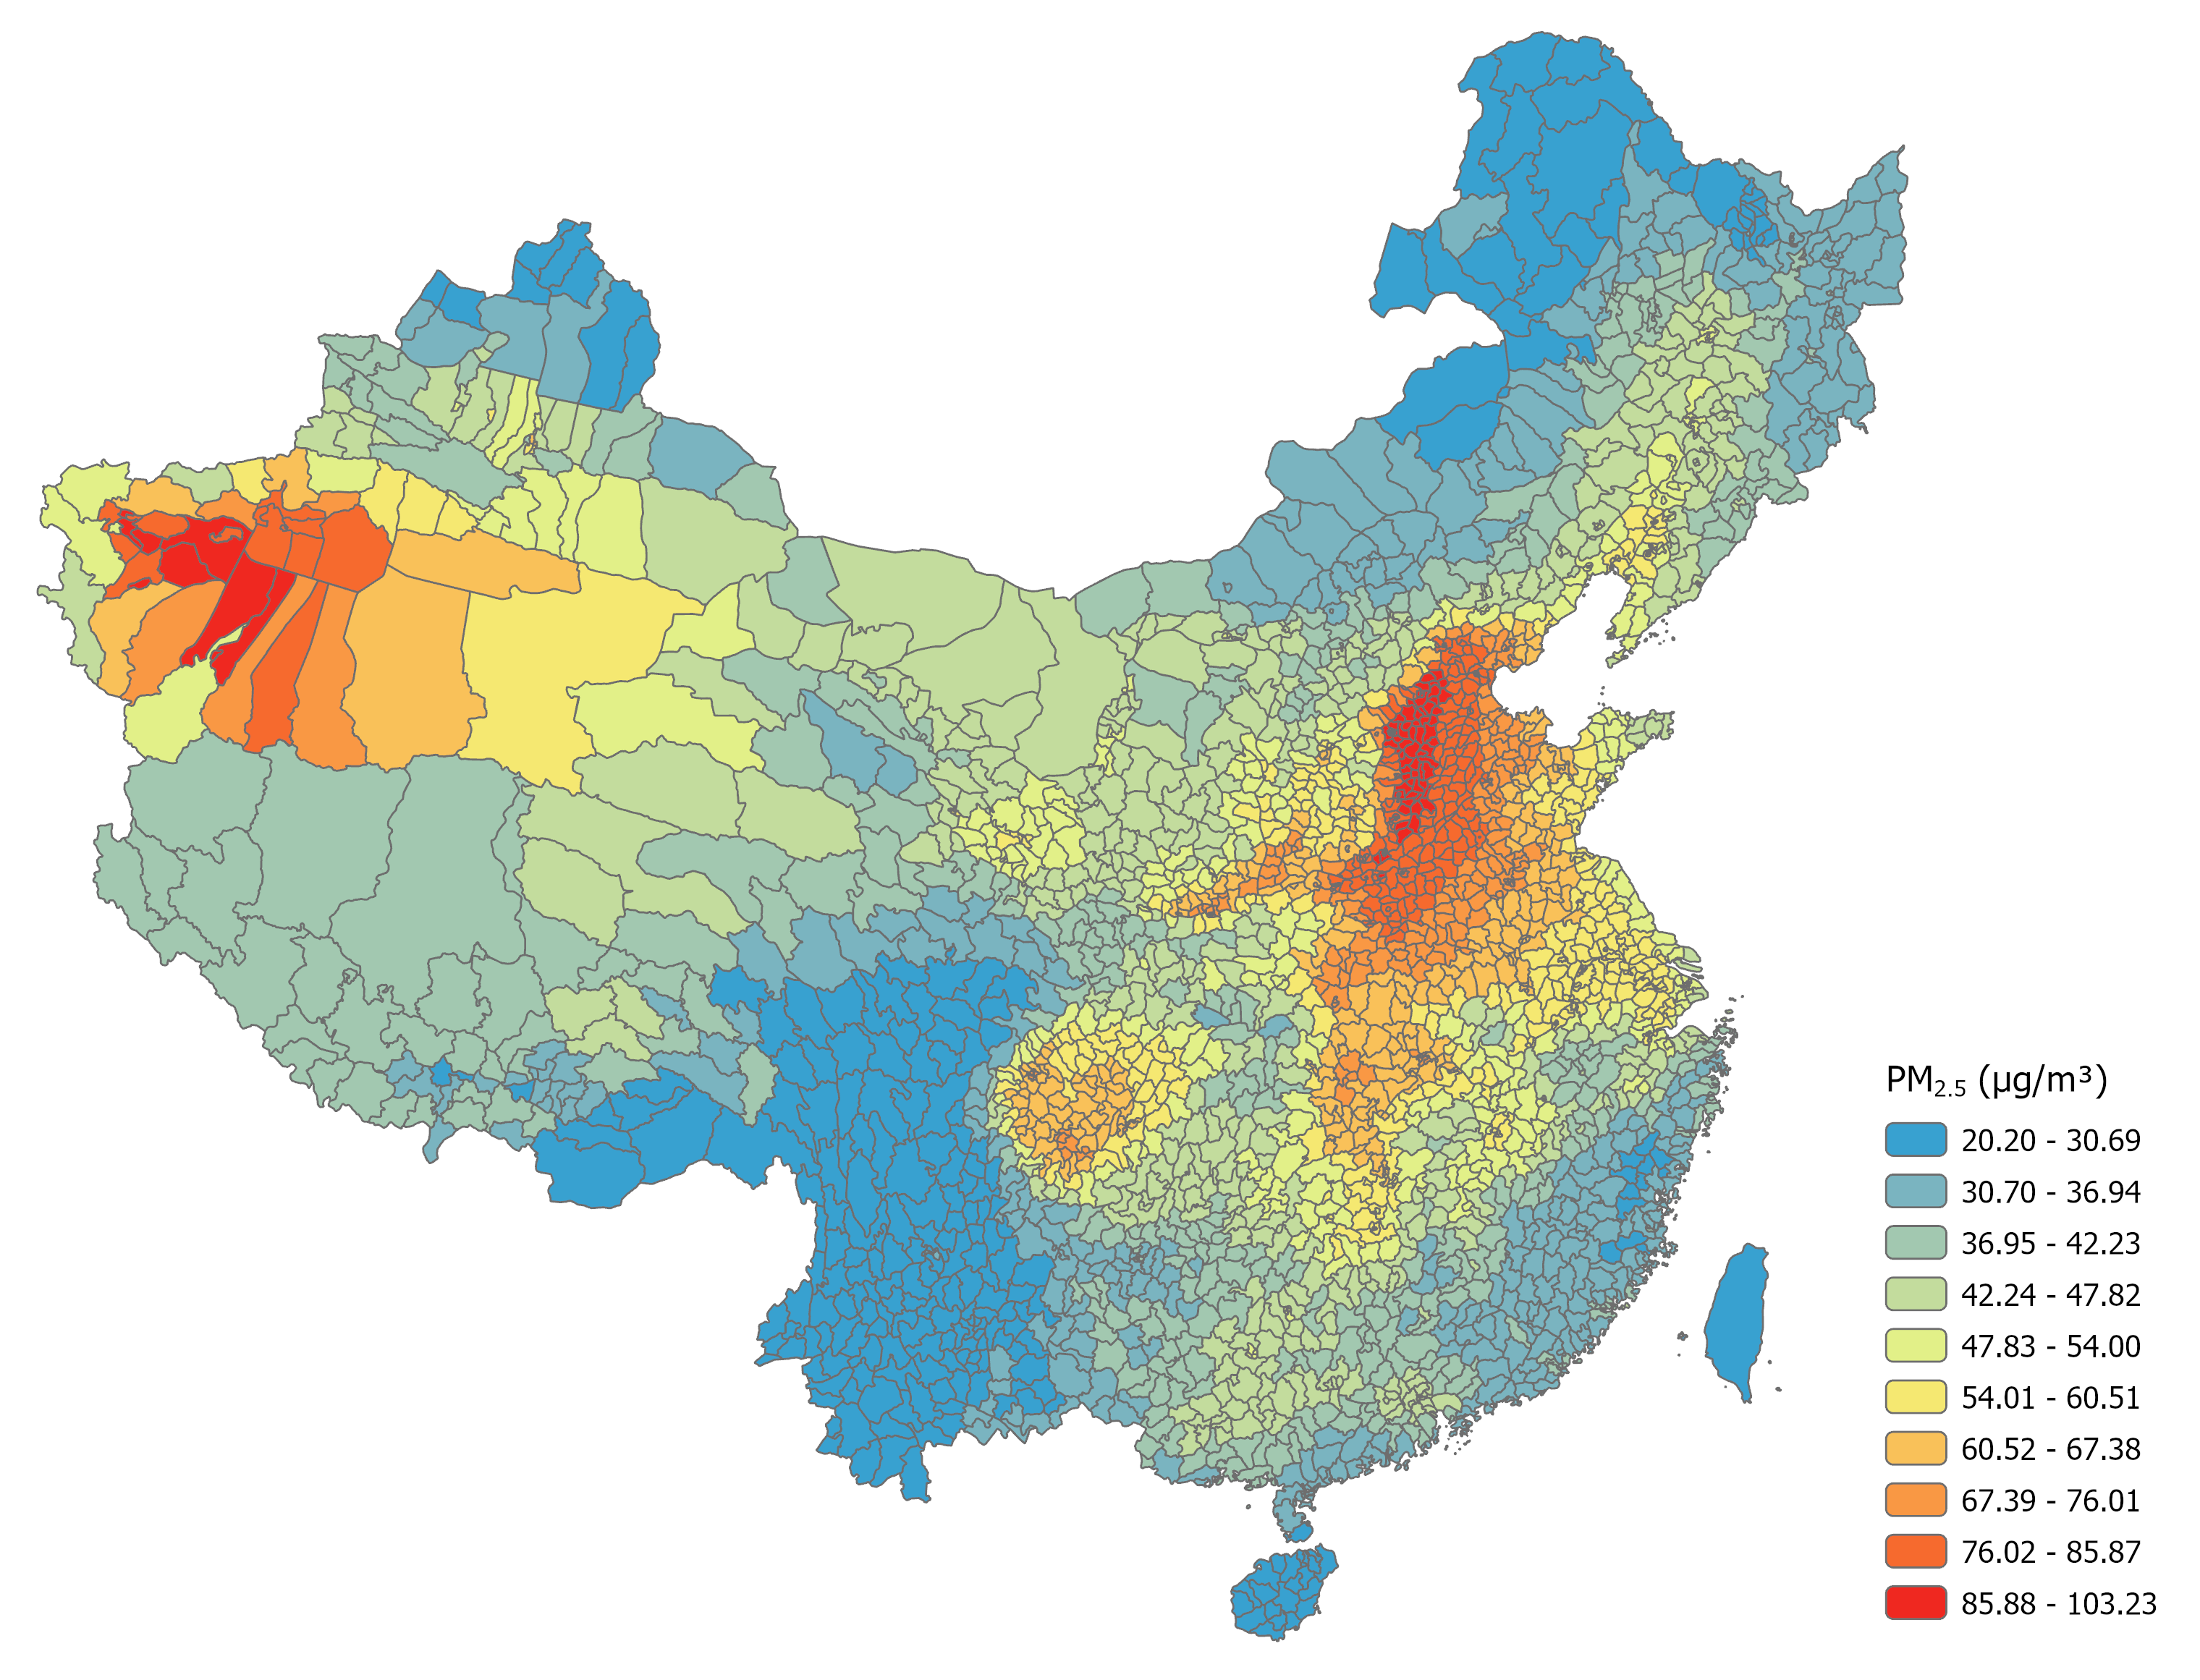
\includegraphics[width=0.85\textwidth]{images_updated/pm00-07}
\end{figure}

\newpage
 \thispagestyle{empty} 
  \begin{figure}[H]
    \caption{Relationship of Thermal Inversions and $\mathrm{PM_{2.5}}$ Concentrations}\label{fig:3}
    \centering
    \begin{minipage}[b]{0.75\textwidth}
      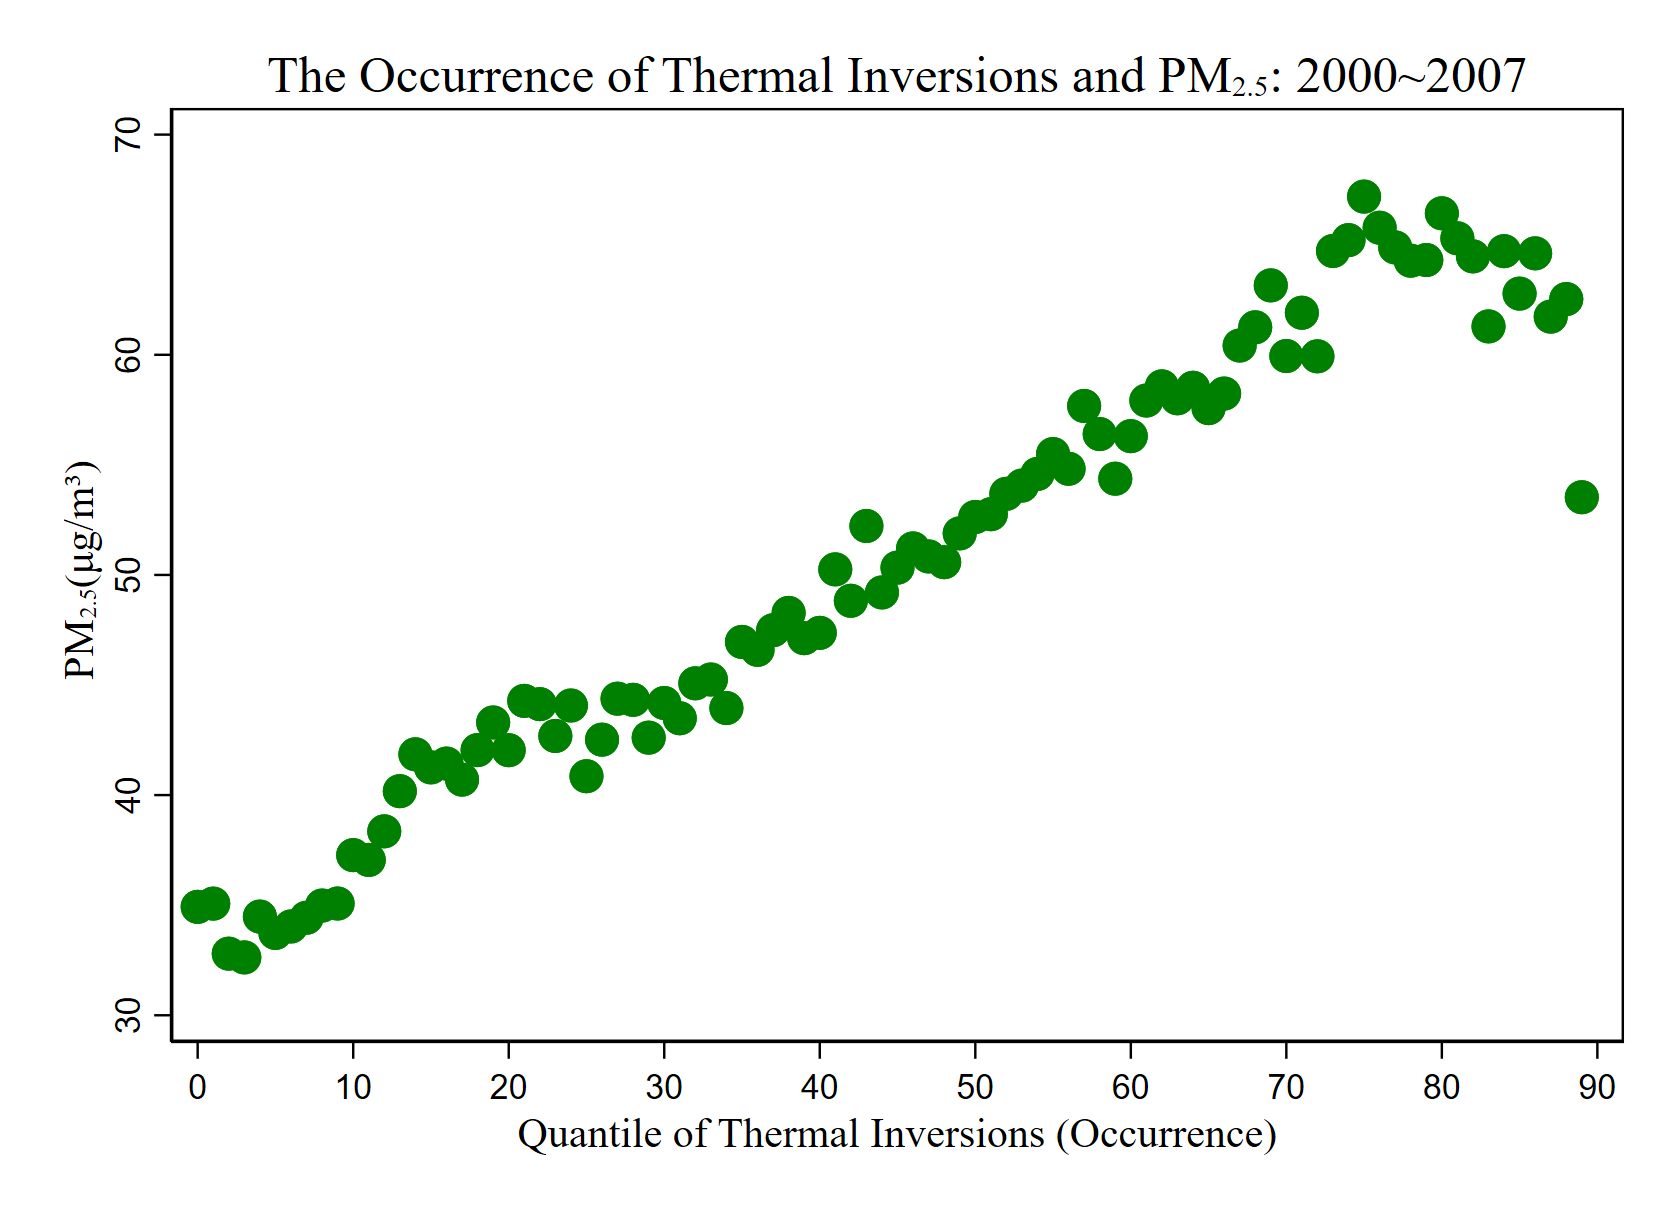
\includegraphics[width=\textwidth]{images_updated/TI_PM2.5_corr.png}
    \end{minipage}
    \centering
    \begin{minipage}[b]{0.75\textwidth}
      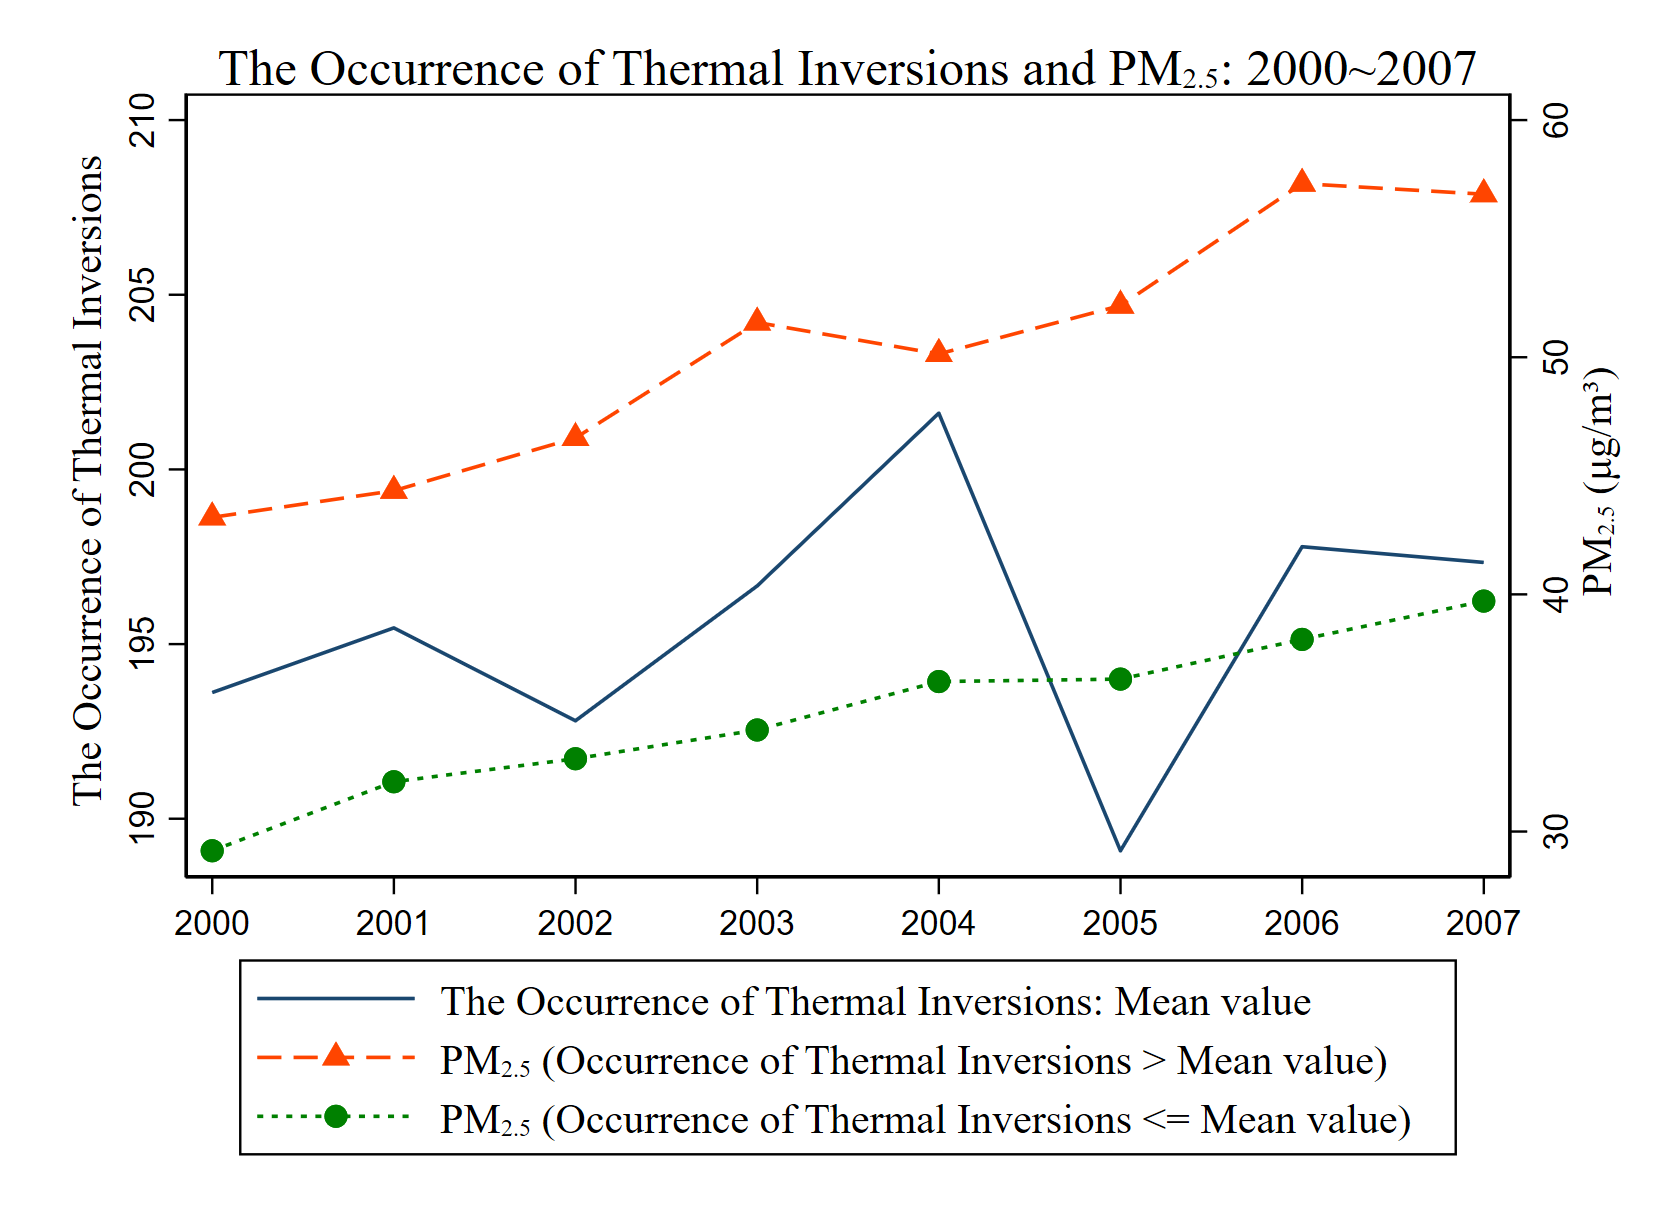
\includegraphics[width=\textwidth]{images_updated/TI_PM25_2.png}
    \end{minipage}
    \small
    \caption*{Notes: In the top panel, counties are divided into 90 quantiles based on the distribution of annual days of thermal inversions. The horizontal axis indicates the annual days of thermal inversions in each quantile. The vertical axis indicates the mean value of $\rm PM_{2.5}$ concentrations in each quantile. The bottom panel shows the occurrence days of thermal inversions from year 2000 to 2007 and annual average $\rm PM_{2.5}$ concentrations in two thermal-inversion groups. Counties are divided into two groups. The blue solid line plots the average annual occurrence in days of thermal inversions over counties from year 2000 to 2007. The red dash line marked with triangle plots the average annual $\rm PM_{2.5}$ of counties whose occurrence of thermal inversions is above the average level and the green dash line marked with dots plots the average annual
    $\rm PM_{2.5}$ of counties whose occurrence of thermal inversions is below the average level.}
  \end{figure}

  \newpage
  \centering
  \begin{figure}[H]
    \centering
     \caption{Trends of PM2.5 and Exports}\label{fig:4}
      \begin{subfigure}[b]{.75\textwidth}
       \centering
        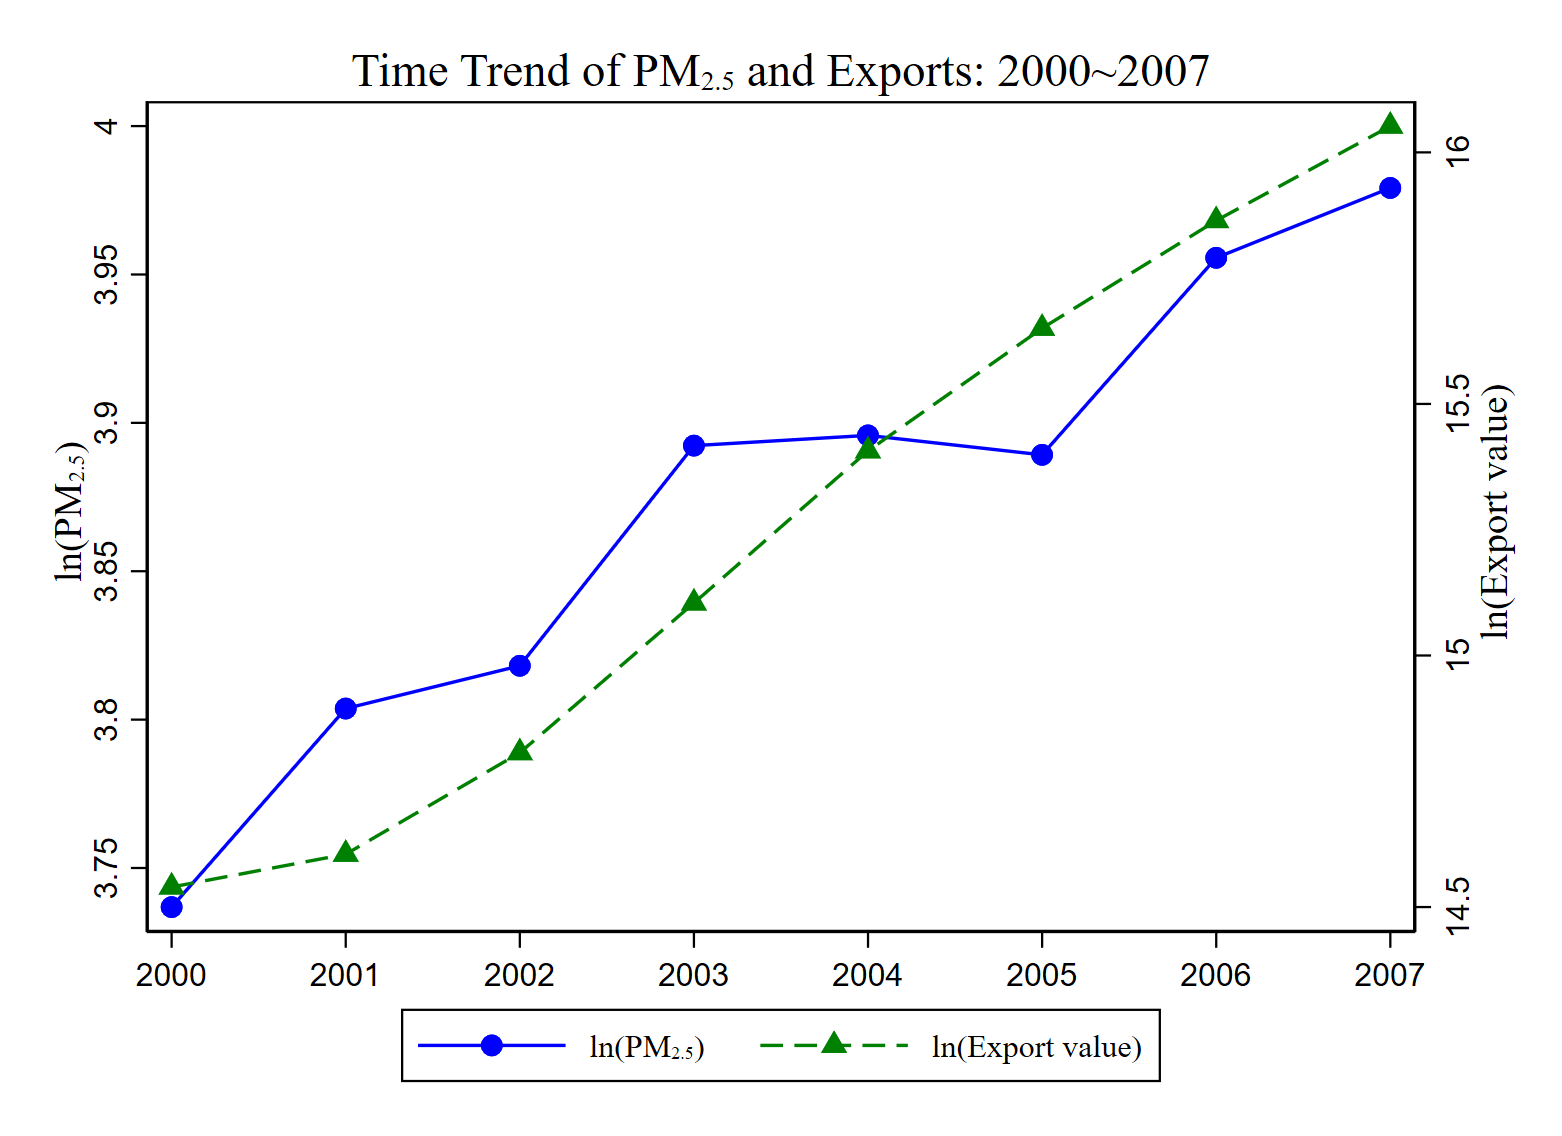
\includegraphics[width=\linewidth]{images_updated/exp_pm25_trend}
        \caption{}\label{fig:fig_4a}
        \end{subfigure}
         \begin{subfigure}[b]{.75\textwidth}
         \centering
         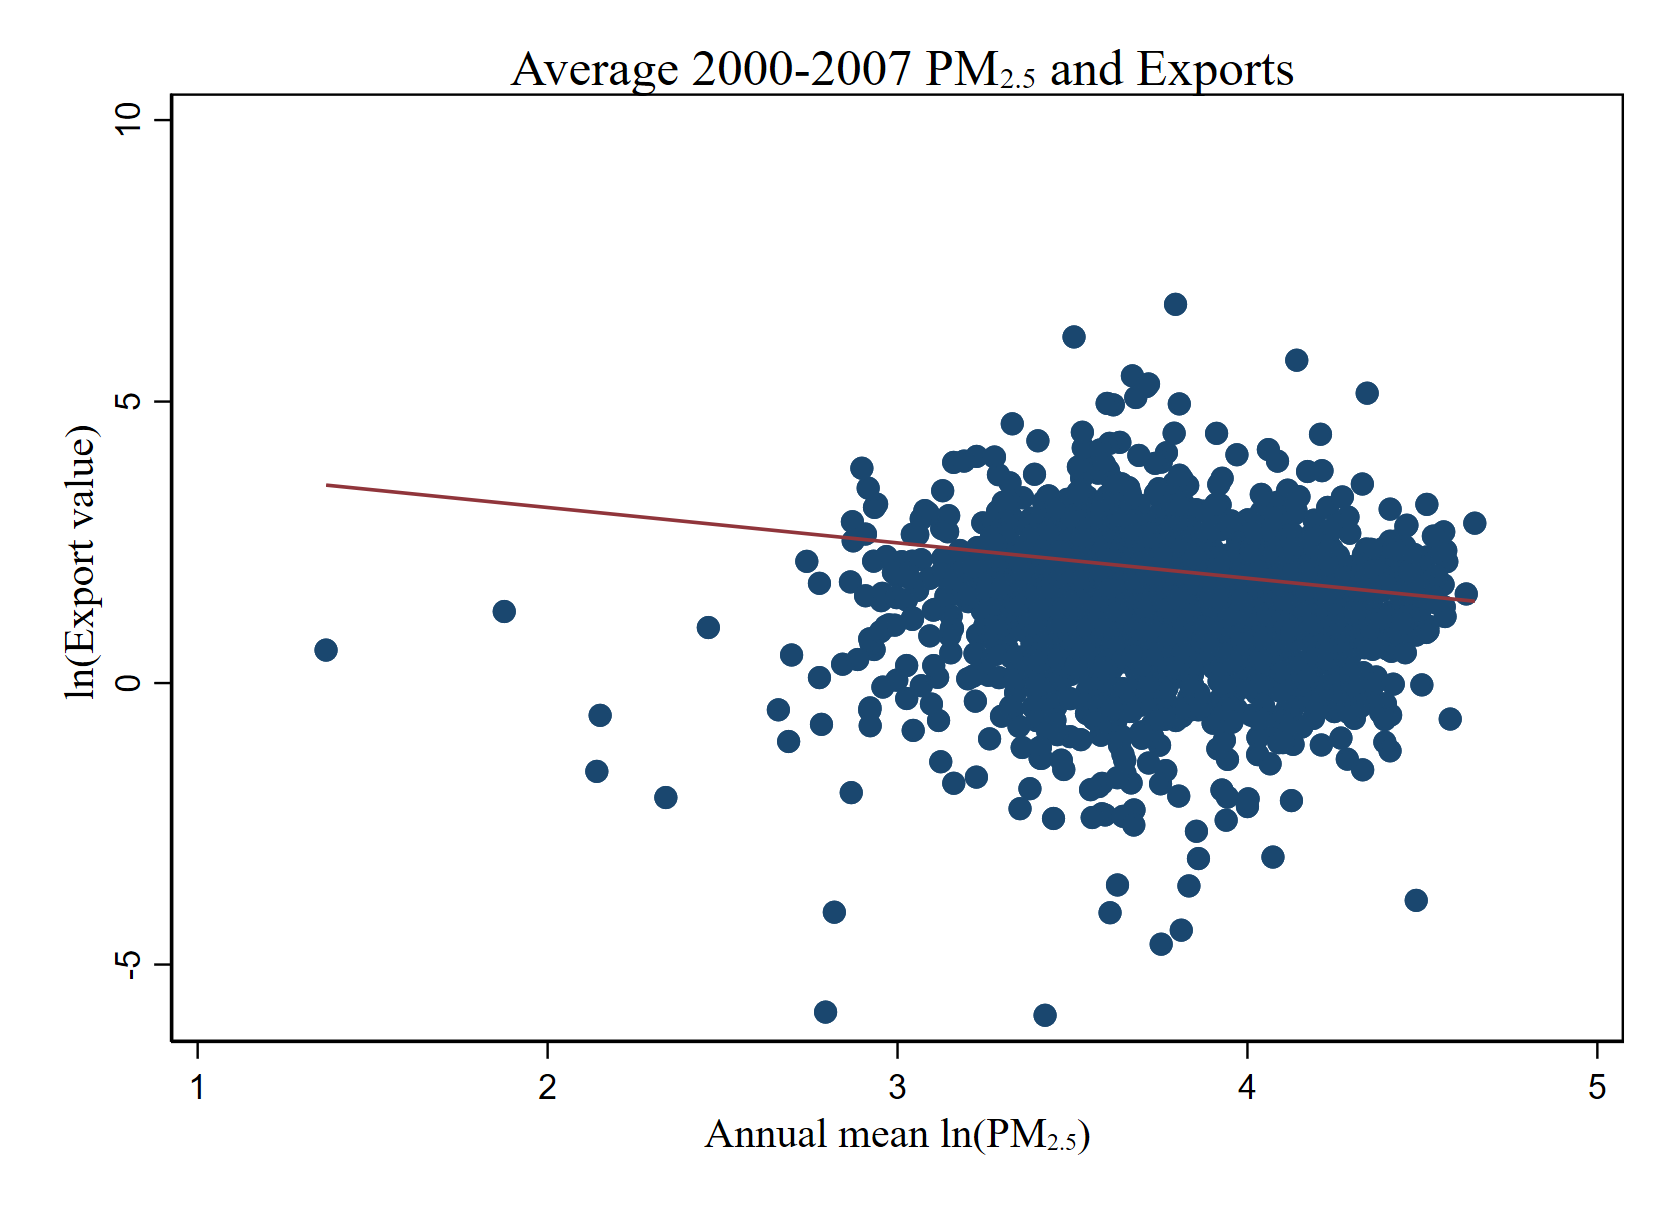
\includegraphics[width=\linewidth]{images_updated/exp_pm25}
          \caption{}\label{fig:fig_4b}
          \end{subfigure}
    \small
    \caption*{Notes: The top panel displays the trend of yearly average $\mathrm{PM_{2.5}}$ ($\mu g/m^3$) and total export value (RMB Million) in China from 2000 to 2007. The bottom panel displays the scatters of the county-level average of $\rm PM_{2.5}$ and exports. The  fitted value line is drawn taking weights by the number of exporters in each county, in case a county with more exporters will be under-represented.}
  \end{figure}
  
%\let\clearpage\relax
\renewcommand \thepart{}
\renewcommand \partname{}
\part{Appendix} % Start the appendix part
\parttoc 
\begin{table}[H]\centering
  \caption{Robustness: firm relocating across counties}
\footnotesize
  \begin{tabular}{l*{6}{c}}
    \hline\hline
    Dep. var.   &$\mathrm{ln(Export)}$&$\mathrm{ln(Export)}$&\multicolumn{2}{c}{Probability of exit}\\
                &\multicolumn{1}{c}{Baseline}&\multicolumn{1}{c}{(1)}&\multicolumn{1}{c}{Baseline}&\multicolumn{1}{c}{(2)}\\
   \hline                    
    $\mathrm{ln(PM_{2.5})}$           &-0.7890***     &-0.8444***	&0.1508**&0.1915***	     \\
                                      &(0.2798)       &(0.3008)	  &(0.0724) &(0.0825)    \\   
    $\mathrm{TFP_{LP}}$, ln           &0.1930***      &0.1925***    &-0.0037*** &-0.0039*** \\
                                      &(0.0045)        &(0.0045)    &(0.0011)&(0.0011)     \\
    Firm age, ln	                  &0.0329***       &0.0349***   &-0.0178***&-0.0182*** \\
                                      &(0.0122)        &(0.0123)    &(0.0037)&(0.0038)	 \\
    Firm size, ln	                  &0.4357***        &0.4353***  &-0.0281***&-0.0280*** \\
                                      &(0.0085) &(0.0085)           &(0.0022)&(0.0022)	 \\
    Firm capital, ln	              &0.1618***&0.1622***          &0.0023& 0.0022	      \\
                                      &(0.0054) &(0.0054)           &(0.0015)&(0.0015)	 \\
                              
    \hline
    Firm FE              &Y&Y&Y&Y\\
    Year FE              &Y&Y&Y&Y\\
    County FE            & &Y&&Y\\
    Weather controls     &Y&Y&Y&Y\\
    KP F-statistic       &4312.80 &7325.55&3133.1&6138.20\\
    Observations         &284,256 &284,251&204,076&204,069  \\
    Firms                &68,002  &68,001 &53,181&53,179      \\
    \hline\hline
  \end{tabular}
\begin{tablenotes}
    \item[*] \small Notes: Estimation method is 2SLS. Weather controls include 20 temperature bins, second-order polynomial in precipitation, humidity, wind speed, and sunshine duration. Standard errors are clustered at firm in parentheses. Statistical significance is denoted by: * p $<$ 0.1, ** p $<$ 0.05, *** p $<$ 0.01.
  \end{tablenotes}
\end{table}
\end{document}

